\documentclass[preprint,12pt]{elsarticle}

\usepackage[T1]{fontenc}
\usepackage[english]{babel}
\usepackage{amsmath,amssymb,amsfonts}
\usepackage{algorithm}
\usepackage{algorithmic}
\usepackage{graphicx}
\usepackage{textcomp}
\usepackage{xcolor}
\usepackage{booktabs}
\usepackage[hidelinks]{hyperref}
\usepackage{titlesec}
\titleformat{\section}{\normalfont\Large\bfseries}{\thesection}{1em}{}
\titleformat{\subsection}{\normalfont\large\bfseries}{\thesubsection}{1em}{}
\titleformat{\subsubsection}{\normalfont\normalsize\bfseries}{\thesubsubsection}{1em}{}
\newcommand{\rvr}{\textsuperscript{$\dagger$}}

% Target venue to be confirmed by the authors (e.g. International Journal of Accounting Information Systems).
\journal{International Journal of Accounting Information Systems}

\begin{document}

\begin{frontmatter}

\title{Leveraging Business Analytics for Audit and Fraud Detection: A Review of Digital Tools and Red-Flag Indicators, with an Empirically Validated AI-Assisted Prioritisation Architecture}

\author[1]{Author Name}
\address[1]{Department, Institution, City, Country}
\cortext[cor1]{Corresponding author. Email: author@example.com}

\begin{abstract}
The growing complexity and digital evolution of financial systems have exposed significant shortcomings in traditional auditing techniques, particularly in identifying and mitigating intricate fraud schemes. This study examines how business analytics improves contemporary audit functions by enhancing fraud detection, increasing audit efficiency and facilitating predictive, real-time assurance across different institutional contexts. A qualitative integrative-review methodology -- thematic synthesis, comparative analysis and typological classification -- was applied to 84 peer-reviewed articles, industry reports and professional publications drawn from five major academic databases (Scopus, Web of Science, IEEE Xplore, SSRN and Google Scholar) and covering 2015--2025, to examine analytical tools, organisational readiness and sector-specific implementations of audit analytics. Anomaly detection, predictive modelling, clustering algorithms and machine learning are analysed for their reported efficacy in detecting atypical financial transactions, behavioural irregularities and structural discrepancies, and the review synthesises a five-cluster red-flag taxonomy, a comparative analysis of five audit-analytics platforms and an analytics-maturity model. Building on this synthesis, the paper proposes a composite AI-assisted red-flag prioritisation framework and, to move beyond a purely conceptual proposal, operationalises it with concrete, reproducible features and empirically calibrates and benchmarks it on a public transaction-level fraud-detection dataset (284,807 European card transactions, 492 confirmed fraud cases). Two instantiations are evaluated -- EC-ARP, a logistic-regression calibration of the proposed formula, and EC-ARP+, a stacked hybrid extension adding a supervised gradient-boosted signal -- against four baselines mirroring techniques reported individually in the reviewed literature (logistic regression, random forest, XGBoost, isolation forest). On a held-out test split, XGBoost attains the highest ranking performance (PR-AUC = 0.842); EC-ARP+ is competitive (PR-AUC = 0.811) and converges with the supervised baselines at the audit-relevant top-1\% investigation-capacity threshold, while the unsupervised, literally-conceptual instantiation (EC-ARP) under-performs (PR-AUC = 0.180). These results are reported candidly, including where the proposed architecture does not exceed simpler baselines, and are discussed as an accuracy-versus-decomposability trade-off relevant to audit practice rather than a claim of superiority. The review also documents ongoing obstacles to analytics adoption -- inconsistent data systems, deficiencies in auditor expertise and ethical concerns around algorithmic bias and insufficient transparency -- and offers a strategic framework for auditors, organisations and regulators to improve digital audit capability. Limitations of both the review (secondary sources, publication and language bias) and the empirical validation (a single public benchmark rather than primary audit-log data, anonymised features, a single train/test split) are reported explicitly, and external validation on primary audit data is identified as a priority for future research. All feature-engineering and model code used to produce the empirical results is released for reproducibility.
\end{abstract}

\begin{keyword}
Business Analytics \sep Audit Automation \sep Fraud Detection \sep Red-Flag Indicators \sep Predictive and Prescriptive Analytics \sep AI-Assisted Prioritisation \sep Ensemble Learning \sep Empirical Validation
\end{keyword}

\end{frontmatter}

\section{Introduction}
\label{sec:intro}

The fast change of financial systems has fundamentally reshaped auditing by producing large quantities of accounting data that cannot easily be processed through traditional audit methods \citep{ebirim2024}. Conventional auditing, based on periodic review cycles, human judgment and selective sampling methods, was designed for a less complex era when financial records were fewer, more stable and less prone to intricate manipulation \citep{darwin2024}. In modern organisations, manual audit methods generally scrutinise only a limited subset of transactions, allowing pervasive fraud in extensive transaction populations to remain undetected for prolonged durations -- frequently months -- before resulting in significant financial loss \citep{rumasukun2024}. These conventional methods have natural limitations in detecting subtle and deliberately concealed alterations in financial records, and therefore do not provide the prompt assurance demanded by a rapidly changing business environment. As financial crime becomes harder to identify because of digital vulnerabilities, complex vendor networks and digital payment systems, traditional audit methods are increasingly insufficient and have become a governance risk in themselves, requiring effective action \citep{johnsonrokosu2025,elumilade2024}.

Business analytics (BA) has emerged as a response to these structural constraints, signifying a transition from reactive, periodic assurance to proactive, continuous and data-driven auditing practices \citep{nouri2024,chowdhury2025}. By facilitating the examination of complete transaction populations instead of samples, BA empowers auditors to uncover anomalies, recognise behavioural irregularities and identify structural flaws in real time. Machine learning algorithms, predictive risk models, network-analysis tools and natural-language-processing capabilities have collectively enhanced auditors' detection capabilities, facilitating the identification of nuanced indicators such as irregular journal-entry patterns, atypical vendor relationships and after-hours system access, which often occur before or alongside fraudulent activity \citep{darwish2024,ilori2024,panchapakesan2025}. The reviewed literature reports that organisations using analytics-driven auditing observe improvements in fraud-detection rates of 30 to 50 percent compared with conventional techniques, alongside a reduction in false-positive rates in anomaly detection attributable to machine-learning optimisation \citep{fernandes2019,johnsonrokosu2025}; these figures come from the cited sources and should be read as reported findings rather than effects independently re-estimated in this review. Overall, these trends indicate that the transition to analytics represents not only a technological enhancement but a substantial advancement in audit efficacy and governance responsibility.

Despite the rising volume of relevant literature, existing research on BA in auditing remains fragmented and insufficiently developed in several critical dimensions. There is a shortage of comparative research assessing the relative effectiveness of different analytical methods -- such as supervised versus unsupervised machine learning -- across audit contexts and fraud types. The literature offers limited guidance on the practical adoption of business analytics within organisations, particularly regarding change management, workflow integration and the development of hybrid competencies that combine accounting proficiency with data-science skills. Much contemporary research also adopts narrow perspectives, focusing on a single technology, an individual industry case, or a technical performance metric considered separately from the organisational and ethical challenges of practical implementation \citep{sewpersadh2025}. Practitioners therefore face legitimate uncertainty about which tools to choose, how to incorporate them into existing audit processes, how to handle algorithmic bias and transparency, and what the enduring effects of analytics adoption are on audit quality and professional scepticism. Without a synthesis that integrates these different parts, academics and practitioners lack the structured foundation needed to advance analytics adoption responsibly. Critically, where the literature does propose conceptual scoring or prioritisation frameworks, such frameworks are rarely operationalised and tested against a reproducible baseline -- a gap this paper addresses directly for one such framework.

Resolving these shortcomings has significant implications for several stakeholder groups, which motivates this study. The absence of established implementation standards leads to inconsistent adoption strategies and undermines confidence in algorithmic outcomes. The lack of uniform standards for algorithmic auditing presents regulatory challenges as analytics becomes further integrated into global assurance practice. The gap between existing curricula and the hybrid skills required of auditors undermines graduates' readiness for data-driven practice \citep{akula2021}. As stakeholder expectations change and regulatory oversight increases across sectors, strong analytical capability becomes essential to maintaining the relevance and value of audit operations \citep{usul2025}. The scarcity of a connected theoretical framework means that empirical studies in BA and auditing are conducted without a systematic structure, limiting comparability and the advancement of knowledge. This work aims to provide an evidence-based synthesis and, in its second component, an empirical test of one candidate framework.

This study pursues five objectives, formulated as the following research questions:
\begin{itemize}
    \item \textbf{RQ1:} What analytical methodologies are applied in audit practice -- including machine learning algorithms, process mining tools and visualisation platforms -- and what are their individual advantages and limitations, as reported in the literature?
    \item \textbf{RQ2:} How can red-flag indicators be organised into an evidence-based classification -- covering financial irregularities, behavioural patterns and structural imbalances -- that gives auditors a practical framework for checking major issues?
    \item \textbf{RQ3:} How does the adoption of business analytics vary across audit and industry sectors, and what sector-specific patterns, challenges and success determinants can be identified?
    \item \textbf{RQ4:} What technological, organisational and ethical barriers -- such as deficiencies in data quality, lack of competence and issues of algorithmic transparency -- constrain the effective adoption of audit analytics?
    \item \textbf{RQ5:} Can a composite, taxonomy-aligned red-flag prioritisation framework be specified concretely, empirically calibrated on real transaction data, and benchmarked against standard machine-learning baselines, and what does such a validation reveal about the trade-off between interpretability and predictive performance?
\end{itemize}

To address RQ1--RQ4, this study implements a qualitative integrative-review approach, analysing 84 peer-reviewed articles, industry reports and professional publications from five major academic databases -- Scopus, Web of Science, IEEE Xplore, SSRN and Google Scholar -- covering the years 2015 to 2025. An integrative method was applied because of the broad-ranging nature of the literature. The main findings show that although business analytics possesses clear and measurable advantages -- including population-level transaction testing, improved detection accuracy and real-time risk signalling -- its effective application is considerably hindered by data-quality deficiencies, reported as the primary obstacle by a majority of organisations in the cited source \citep{wolniak2024}, skill gaps affecting audit teams \citep{vesty2023}, and persistent ethical issues surrounding AI-based insight and imbalance \citep{landers2023}. Adoption rates differ markedly across sectors: financial institutions report substantially higher adoption, primarily due to regulatory pressure, while small and medium-sized enterprises report much lower adoption, mainly attributable to resource and capacity constraints \citep{kothandapani2025,fiolleau2024}. Forensic investigations are reported to be enhanced by network-analysis skills \citep{hezam2023}, and regulators are reported to be progressively adopting business analytics for systemic risk monitoring and compliance trend analysis \citep{syam2025}.

To address RQ5, Section~\ref{sec:framework} proposes a composite, model-agnostic AI-assisted red-flag prioritisation framework that consolidates the taxonomy and workflow synthesised from the review, and Section~\ref{sec:empirical-method} operationalises and empirically validates it. Consistent with the review's own emphasis on avoiding overclaiming, the validation results are reported candidly in Section~\ref{sec:empirical-results}: the proposed stacked hybrid model is competitive with, but does not exceed, a plain gradient-boosted baseline on raw ranking metrics, while the purely unsupervised instantiation of the framework under-performs.

This research provides several contributions to audit scholarship and practice:
\begin{itemize}
    \item \textbf{C1:} a documented, PRISMA-informed review protocol synthesising 84 sources on business analytics in auditing into a coherent account, positioning analytics as an enabler of proactive, risk-oriented assurance.
    \item \textbf{C2:} an evidence-based, five-cluster taxonomy of red-flag indicators, linked to the analytical techniques reported to detect each cluster.
    \item \textbf{C3:} a comparative synthesis of five audit-analytics platforms and an analytics-maturity model connecting descriptive-to-prescriptive capability with organisational conditions.
    \item \textbf{C4:} a composite, model-agnostic AI-assisted red-flag prioritisation framework, proposed in this paper and expressed as an interpretable weighted risk score.
    \item \textbf{C5:} an open, reproducible empirical validation of the C4 framework -- two concrete instantiations, EC-ARP and EC-ARP+ -- feature-engineered and benchmarked against four standard baselines on a public 284,807-transaction fraud-detection dataset, with code, results and calibrated weights released so the validation can be audited and extended to primary audit data.
\end{itemize}

The remainder of the paper is organised as follows. Section~\ref{sec:method} describes the review methodology, the proposed prioritisation framework, and the empirical validation design. Section~\ref{sec:results} synthesises the review findings and reports the empirical validation results. Section~\ref{sec:ethics} discusses ethical considerations. Section~\ref{sec:conclusion} presents conclusions, policy recommendations and limitations.

\section{Methodology}
\label{sec:method}

This study provides a structured qualitative approach to evaluate the impact of business analytics on auditing and fraud detection, complemented by a quantitative empirical validation of one proposed framework. The qualitative component enables the systematic identification and evaluation of digital technologies, auditing procedures and fraud indicators through comparative and thematic analysis, integrating theoretical insight with practical evidence. Given the transdisciplinary nature of the research problem, this study adopts an integrative-review technique rather than a systematic review, emphasising synthesis over data pooling. A PRISMA-informed screening structure was applied during literature selection to improve transparency and rigour.

\subsection{Research Design and Analytical Strategy}

The review implements a qualitative, exploratory and integrative design to synthesise mixed information sources on audit innovation, fraud detection and business analytics, aiming to derive conceptual patterns and operational principles from the literature and industry practice without depending on a fixed a priori model. The interpretive lens adopted holds that audit tools and red-flag indicators acquire meaning and effectiveness through their positioning within distinct institutional, technological and cultural configurations -- that is, audit technologies evolve in response to localised institutional demands and sociocultural influences rather than in a vacuum. The integrative design allows the inclusion of empirical studies, theoretical frameworks, grey literature and industry reports, facilitating the exploration of emerging trends and practical challenges through narrative and comparative synthesis.

\subsection{Literature Search and Source Selection}

A multi-stage retrieval technique was used to compile an extensive body of academic and professional literature on audit analytics and fraud-detection systems. A purposive sampling strategy was applied and enhanced by iterative refinement of search terms to ensure thematic accuracy. Keywords encompassed ``audit automation'', ``fraud analytics'', ``continuous auditing'', ``anomaly detection in finance'' and ``digital auditing frameworks'', among other pertinent terms. Academic resources were retrieved from five primary databases: Scopus ($n=64$), Web of Science ($n=41$), IEEE Xplore ($n=36$), SSRN ($n=58$) and Google Scholar ($n=73$). Additionally, 25 documents from industry reports and white papers released by ISACA and the Big Four accounting firms were incorporated to combine academic rigour with practical applicability. Inclusion criteria required methodological transparency, relevance to digital auditing or fraud analytics, and practical usefulness to organisational decision-making; editorial documents lacking clarity of execution or focused on non-financial aspects were excluded. After examination of titles, abstracts and full texts, 84 pertinent sources were retained from an original pool of 297 records. Table~\ref{tab:protocol} summarises each screening stage.

% [AUTHOR INPUT REQUIRED: insert the exact database search strings and the date of the final search.]
% [AUTHOR INPUT REQUIRED: state whether screening was performed by one reviewer or independently by multiple reviewers, and inter-rater agreement if applicable.]
% [AUTHOR INPUT REQUIRED: state the screening/reference-management software used and the final split of the 84 sources into peer-reviewed vs industry/professional.]

\begin{table}[!t]
\caption{Literature Screening and Selection Process}
\label{tab:protocol}
\centering
\footnotesize
\begin{tabular}{p{0.40\columnwidth} p{0.15\columnwidth} p{0.28\columnwidth}}
\toprule
\textbf{Screening phase} & \textbf{Count} & \textbf{Overview} \\
\midrule
Total records initially retrieved & 297 & Scopus, Web of Science, IEEE Xplore, SSRN, Google Scholar and industry sources \\
Duplicates eliminated & 25 & Redundant entries across databases \\
Records post-de-duplication & 272 & Distinct titles eligible for screening \\
Excluded following title/abstract review & 118 & Irrelevant subjects or non-academic material \\
Excluded after full-text evaluation & 70 & Editorials, absence of methodological rigour, or unrelated to finance \\
Final records incorporated & 84 & Fulfilled all inclusion criteria \\
\bottomrule
\end{tabular}
\end{table}

The chosen documents illustrate a range of contributions, including theoretical frameworks, empirical research, applied machine-learning methodologies and practical case studies. To assist synthesis, sources were clustered into three groups: (1) theoretical frameworks, (2) empirical research, and (3) technical or industry reports. This classification corresponded to the interpretive philosophical stance of the review and provided a basis for analysing red-flag indicators, uptake of audit-data systems and practical integration of audit technologies by merging academic material with practitioner-oriented views.

\subsection{Comparative Framework for Audit Models}

This assessment compares audit models using five key dimensions -- data coverage, audit timing, fraud-detection agility, workforce efficiency and anomaly traceability -- obtained from recognised literature and industry standards and used as coding categories for classifying the selected sources during thematic synthesis. Table~\ref{tab:framework} outlines the resulting attributes of traditional and analytics-driven auditing. Each evaluated source was assessed against this consistent set of criteria, enabling cross-comparison and the identification of transition patterns from traditional to analytics-enabled audit processes.

\begin{table}[!t]
\caption{Comparative Framework: Conventional versus Analytics-Enabled Auditing}
\label{tab:framework}
\centering
\footnotesize
\begin{tabular}{p{0.18\columnwidth} p{0.33\columnwidth} p{0.33\columnwidth}}
\toprule
\textbf{Aspect} & \textbf{Conventional auditing} & \textbf{Analytics-based auditing} \\
\midrule
Data volume scope & Depends on sample-based evaluation, providing restricted understanding. & Encompasses complete datasets, facilitating thorough analysis \citep{faccia2024}. \\
Frequency of audits & Executed at regular intervals, usually annually or quarterly. & Facilitates continuous or near-real-time auditing procedures \citep{hassan2023}. \\
Detection response & Discerns problems post-occurrence, leading to reactive interventions. & Facilitates real-time or predictive identification for pre-emptive measures \citep{adepoju2022}. \\
Resource allocation & Labour-intensive and manual, requiring considerable human involvement. & Automated and systematised, diminishing manual labour \citep{vajpayee2023}. \\
Fraud tracking & Insufficient traceability due to inconsistent documentation. & Enhanced traceability through fully auditable digital records \citep{prosper2025}. \\
\bottomrule
\end{tabular}
\end{table}

Throughout the evaluation process, each source was analysed for the degree of alignment between its articulated audit methodology and the criteria in Table~\ref{tab:framework}, with occurrences of convergence or integration between conventional and analytics-based attributes documented for later synthesis. This procedure reduced interpretive bias and linked subsequent findings to a transparent comparison framework, moving the review from descriptive comparison to a reproducible, evidence-based approach for evaluating the uptake and effects of analytics in auditing.

\subsection{Tool Categorisation and Functional Analysis}

A review was undertaken to identify the functional capabilities of common business-analytics solutions, concentrating on five tools and platforms recognised as key in academic and commercial literature: ACL, IDEA, Power BI, Tableau, and open-source solutions (Python and R). Table~\ref{tab:tools} compares these platforms across four dimensions reported consistently across the literature.

\begin{table}[!t]
\caption{Comparative Analysis of Audit Analytics Tools}
\label{tab:tools}
\centering
\scriptsize
\setlength{\tabcolsep}{4pt}
\resizebox{\textwidth}{!}{%
\begin{tabular}{p{0.08\textwidth} p{0.20\textwidth} p{0.20\textwidth} p{0.20\textwidth} p{0.22\textwidth}}
\toprule
\textbf{Tool} & \textbf{Data integration} & \textbf{Visualisation strength} & \textbf{Fraud-detection effectiveness} & \textbf{Ease of learning / adoption} \\
\midrule
ACL & Moderate capacity for integrating diverse datasets. & Basic visual-representation features. & Moderate utility in detecting irregularities. & Low -- user-friendly for beginners \citep{pamisetty2021}. \\
IDEA & High-level data integration across formats. & Adequate visualisation capability. & Strong suitability for fraud identification. & Moderate -- requires some training \citep{hamdam2022}. \\
Power BI & Robust integration with multiple data sources. & High-quality, interactive visuals. & Moderately effective for anomaly detection. & Low -- relatively easy to learn \citep{abdelwahed2024}. \\
Tableau & Robust, seamless data-connection features. & Very high visual-analytics strength. & Limited direct utility for fraud detection. & Low -- intuitive for new users \citep{thakkar2025}. \\
Python / R & Exceptionally strong and scalable integration. & Fully customisable, highly flexible. & Very high efficacy in complex fraud analytics. & High -- steep learning curve \citep{pinto2024}. \\
\bottomrule
\end{tabular}%
}
\end{table}

This comparison shows a distinct trade-off between power and accessibility: Python and R emerge as the most effective platforms for integration and sophisticated fraud detection, guiding the emphasis on advanced analytical capability in the thematic synthesis, while Tableau and Power BI are classified as strong in visualisation and accessibility. No single tool is suitable in every context, motivating context-specific tool selection.

\subsection{Workflow Model of Analytics-Driven Audit Lifecycle}
\label{sec:workflow}

The reviewed sources converge on a five-stage continuum depicting the increasingly significant role of analytics in modern audit operations: data collection, data preparation (pre-audit configuration), exploratory modelling, risk assessment and red-flag generation. Every phase involves a combination of dedicated resources and audit-relevant skills mapped to that function's operational requirements. Data collection acquires structured and unstructured financial data from enterprise resource planning (ERP) systems, spreadsheets, transaction logs and internal communications. Data preparation concentrates on cleansing, redundancy elimination, transformation and normalisation, so that datasets are accurately formatted for audit and analytics purposes; the reviewed sources describe this stage as the most resource-intensive of the workflow. Exploratory modelling leverages clustering algorithms, trend-detection mechanisms and outlier-identification techniques to uncover hidden relationships and irregularities. Risk scoring assigns weighted values to the frequency and severity of anomalies, enabling auditors to rank investigative tasks by urgency and relevance. The concluding phase, red-flag issuance, produces alerts and visual summaries incorporated into auditor dashboards for prompt decision-making. This cycle functions as an ongoing loop rather than a fixed sequence: insights from red-flag outputs frequently guide modifications to preceding stages, such as enhancing data features or calibrating model parameters, and embedding governance tools improves alignment between audit analytics and organisation-wide risk protocols. Figure~\ref{fig:workflow} presents this workflow.

\begin{figure}[!t]
\centering
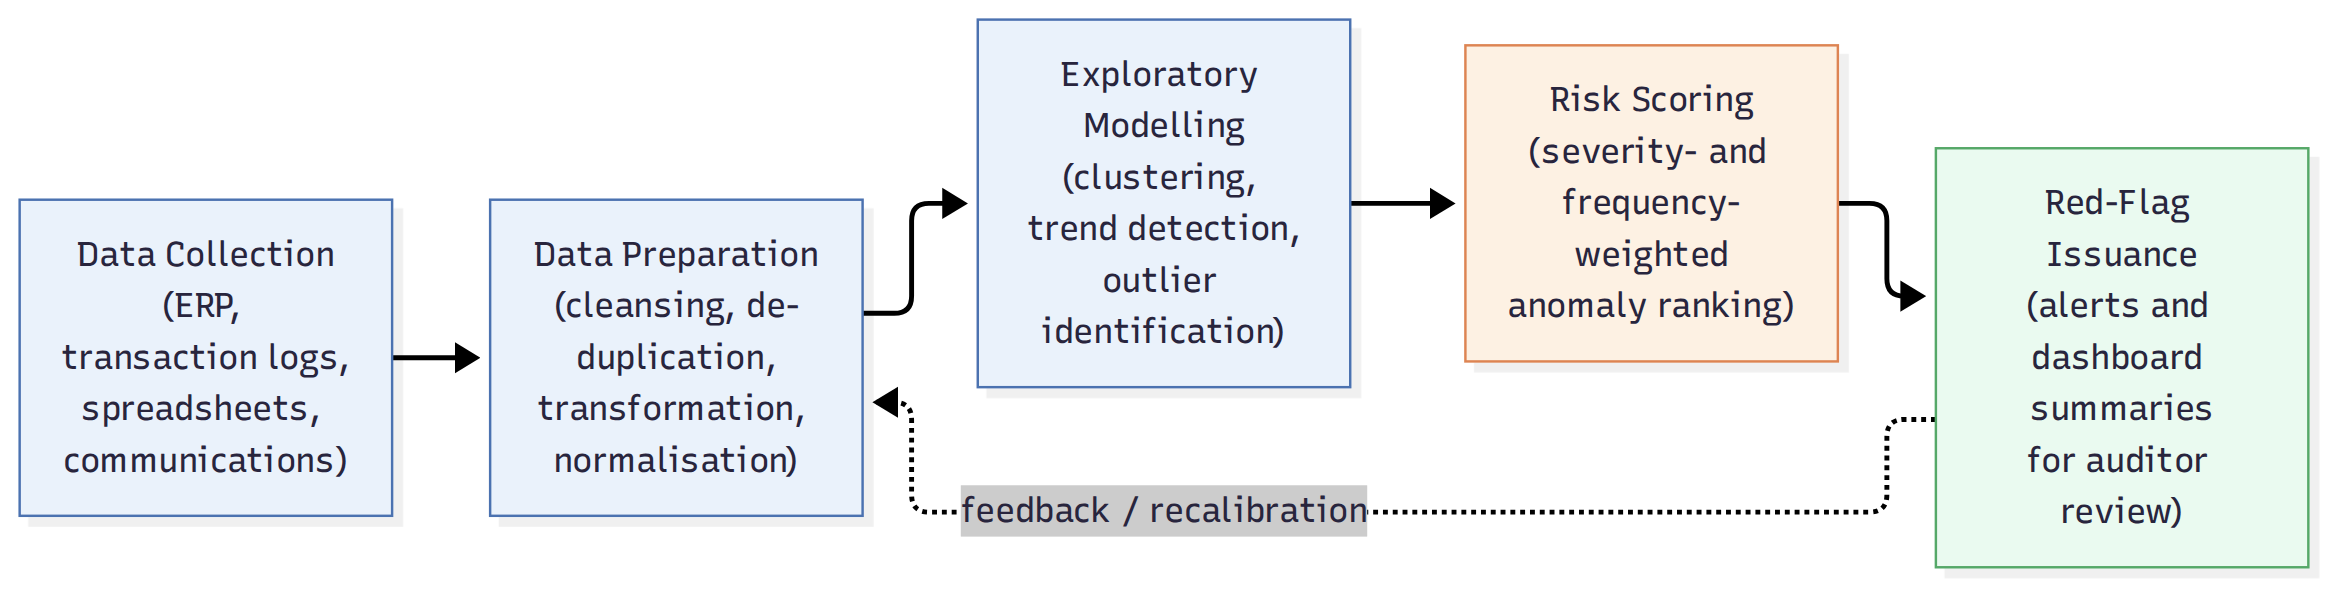
\includegraphics[width=\columnwidth]{figs/mermaid_workflow.png}
\caption{Analytics-driven audit and fraud-detection workflow. Data preparation is reported by the reviewed sources as the most resource-intensive phase; the cycle operates as a feedback loop rather than a strict linear sequence.}
\label{fig:workflow}
\end{figure}

\subsection{Extraction and Typological Classification of Red-Flag Indicators}
\label{sec:taxonomy}

Efficient fraud detection relies on promptly recognising warning signs, generally known as red-flag indicators. This review classifies indicators into five clusters, organised by their complexity and the traceability of their underlying data sources: transaction irregularities (e.g., duplicate transactions or payments executed outside business hours), behavioural anomalies (e.g., recurrent violations of internal controls), structural anomalies (e.g., unbalanced ledger accounts or incongruous reconciliations), documentation discrepancies (e.g., altered, counterfeit or duplicated invoices), and relational fraud patterns (e.g., indications of coordination or synchronised fraudulent activity among entities). Figure~\ref{fig:taxonomy} presents this taxonomy. Each cluster is associated with particular analytical techniques -- for example regression models, clustering algorithms or relational network analysis -- contingent on the characteristics and complexity of the identified patterns. This stratified approach improves the precision of model selection and equips auditors to prioritise risks by associating specific red-flag signs with specific fraud schemes, so that high-risk situations receive prompt and appropriate investigative attention.

\begin{figure}[!t]
\centering
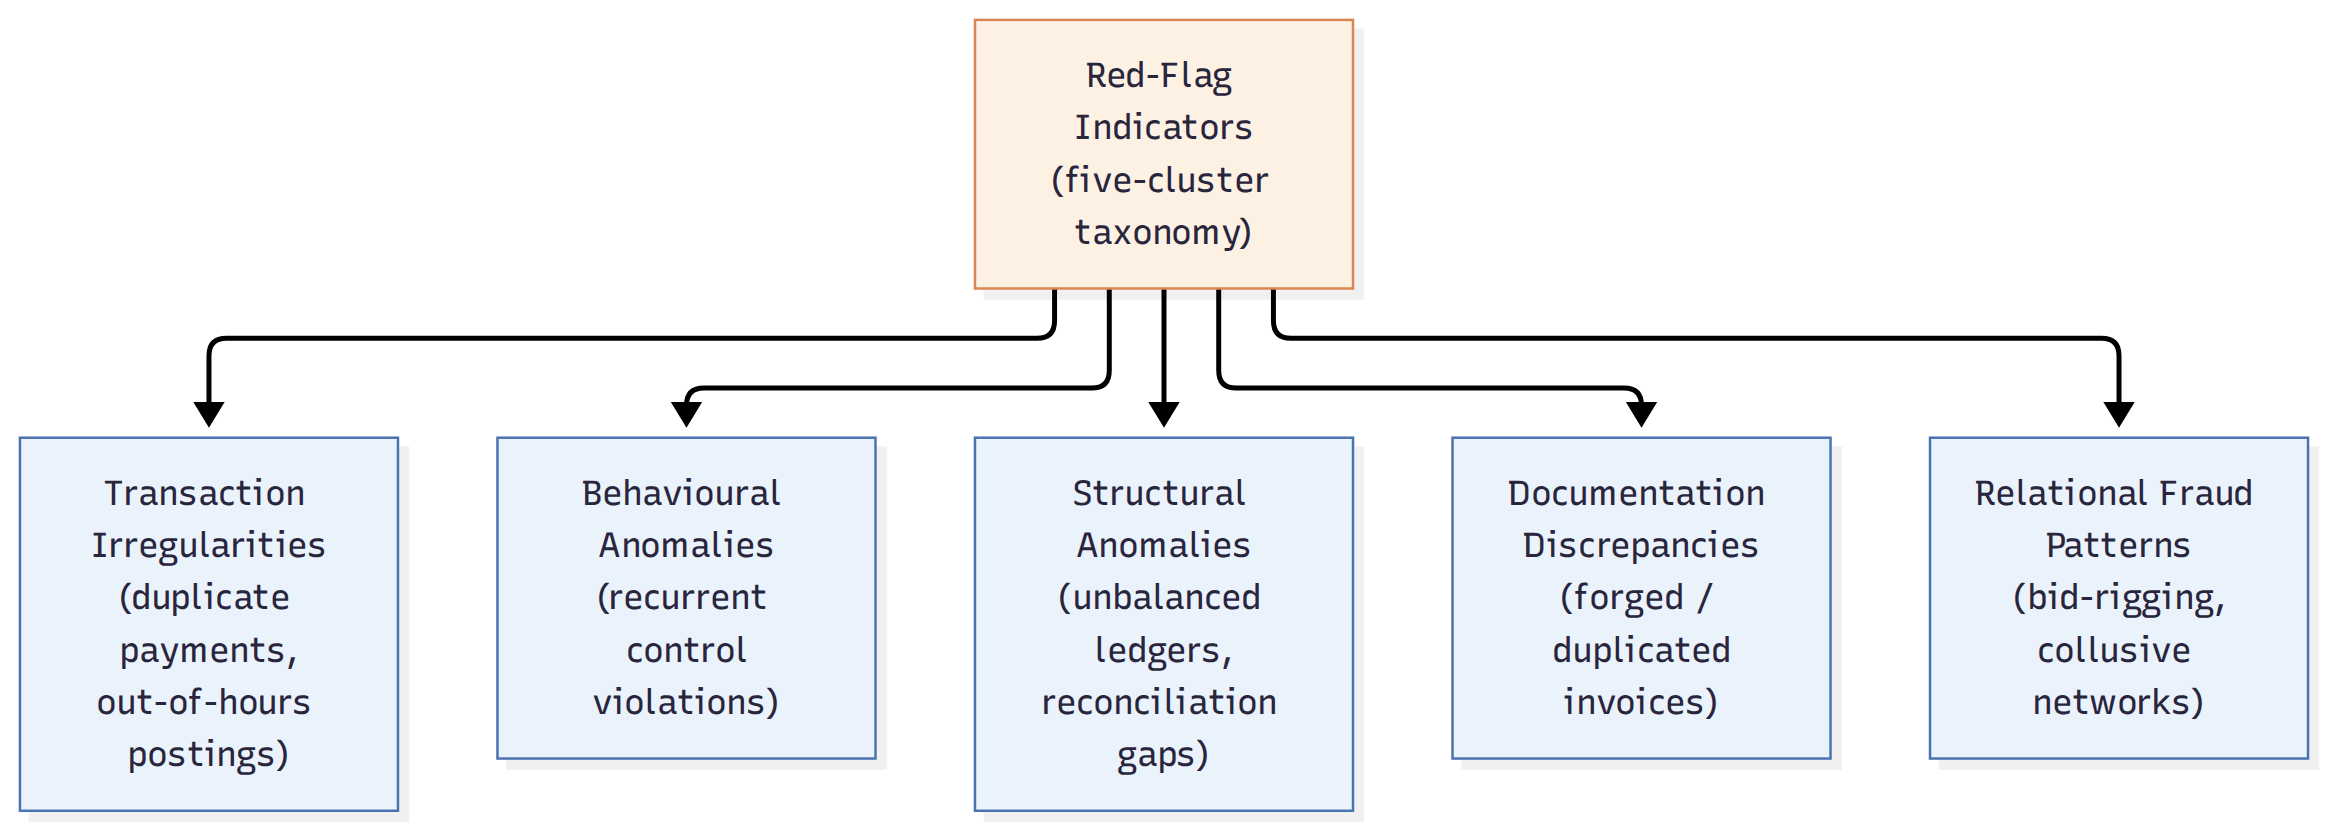
\includegraphics[width=\columnwidth]{figs/mermaid_taxonomy.png}
\caption{Five-cluster red-flag indicator taxonomy. Clusters are not assumed to be mutually exclusive; indicators may co-occur across clusters, which motivates the combined prioritisation framework proposed in Section~\ref{sec:framework}.}
\label{fig:taxonomy}
\end{figure}

\subsection{Thematic Synthesis and Validation Protocol}

An inductive thematic-synthesis method, following the three-stage framework established by Thomas and Harden, was used to examine the diverse literature: (1) coding the findings by reading each article line-by-line to extract features pertaining to audit-tool capabilities, alert indicators, implementation challenges and value propositions; (2) formulating descriptive themes through iterative comparative analysis, consolidating preliminary codes into overarching themes; and (3) formulating analytical themes that go beyond description to establish an interpretive framework, identifying links and patterns among descriptive themes that demonstrate the strategic importance of data curation, context-specific tool selection, fraud-pattern modelling and operational integration in audit environments. Further sources added little value once no new themes emerged from additional evidence, and the codebook was cross-reviewed and refined across analytical cycles to improve interpretative reliability across document types and stakeholder perspectives.

Findings were further validated through triangulation: contrasting academic findings with the industry norms and practices of the Big Four firms; verifying that tool functionality corresponded with publicly accessible documentation; and correlating red-flag typologies with case narratives in forensic-accounting reports. This rigorous triangulation aimed to ensure findings were evidence-based and representative of real-world complexities, though it strengthens interpretation rather than converting the synthesis into a controlled empirical validation of the reviewed claims themselves.

\subsection{Proposed AI-Assisted Red-Flag Prioritisation Framework}
\label{sec:framework}

Building on the workflow (Section~\ref{sec:workflow}) and the taxonomy (Section~\ref{sec:taxonomy}), this paper proposes a composite, model-agnostic framework that consolidates the analytical techniques identified in the review into a single interpretable score per transaction or journal entry, so that finite audit resources can be directed towards the most consequential cases. Let $x_r$ denote the feature vector of record $r$ (temporal, monetary, categorical and textual attributes). Four terms are combined, each normalised to $[0,1]$:
\begin{itemize}
    \item $a(x_r)$: an unsupervised anomaly score (for example from an isolation forest, an autoencoder, or a clustering-distance measure);
    \item $b(x_r)$: a behavioural-deviation score relative to a peer group or the entity's own history;
    \item $c(x_r)\in\{0,1\}$: a binary indicator that record $r$ violates a defined control rule;
    \item $f(x_r)$: a normalised frequency/severity term capturing how often and how materially such an event occurs.
\end{itemize}
The composite risk score is
\begin{equation}
s(r)=w_1 a(x_r)+w_2 b(x_r)+w_3 c(x_r)+w_4 f(x_r),
\label{eq:risk}
\end{equation}
where the weights satisfy $w_i \ge 0$ and $\sum_{i=1}^{4} w_i = 1$, so that $s(r)\in[0,1]$ and admits a single interpretable threshold $\tau$: records with $s(r) > \tau$ are escalated for investigation, while records below $\tau$ enter routine monitoring. The framework is intentionally model-agnostic -- each term can be instantiated with statistical, clustering, graph-based or supervised techniques -- allowing model complexity to be matched to an organisation's data and analytical maturity, and it maps directly onto the taxonomy of Section~\ref{sec:taxonomy}: $a$ and $b$ target transaction irregularities and behavioural anomalies, $c$ targets rule-based control violations, and $f$ targets the severity/frequency dimension common to several clusters. As proposed, the weights $w_1$--$w_4$ and the threshold $\tau$ are free parameters requiring calibration on representative data; Section~\ref{sec:empirical-method} performs this calibration empirically rather than leaving the framework purely conceptual. Figure~\ref{fig:architecture} presents the framework together with its empirical instantiation (Section~\ref{sec:empirical-method}).

\begin{figure*}[!t]
\centering
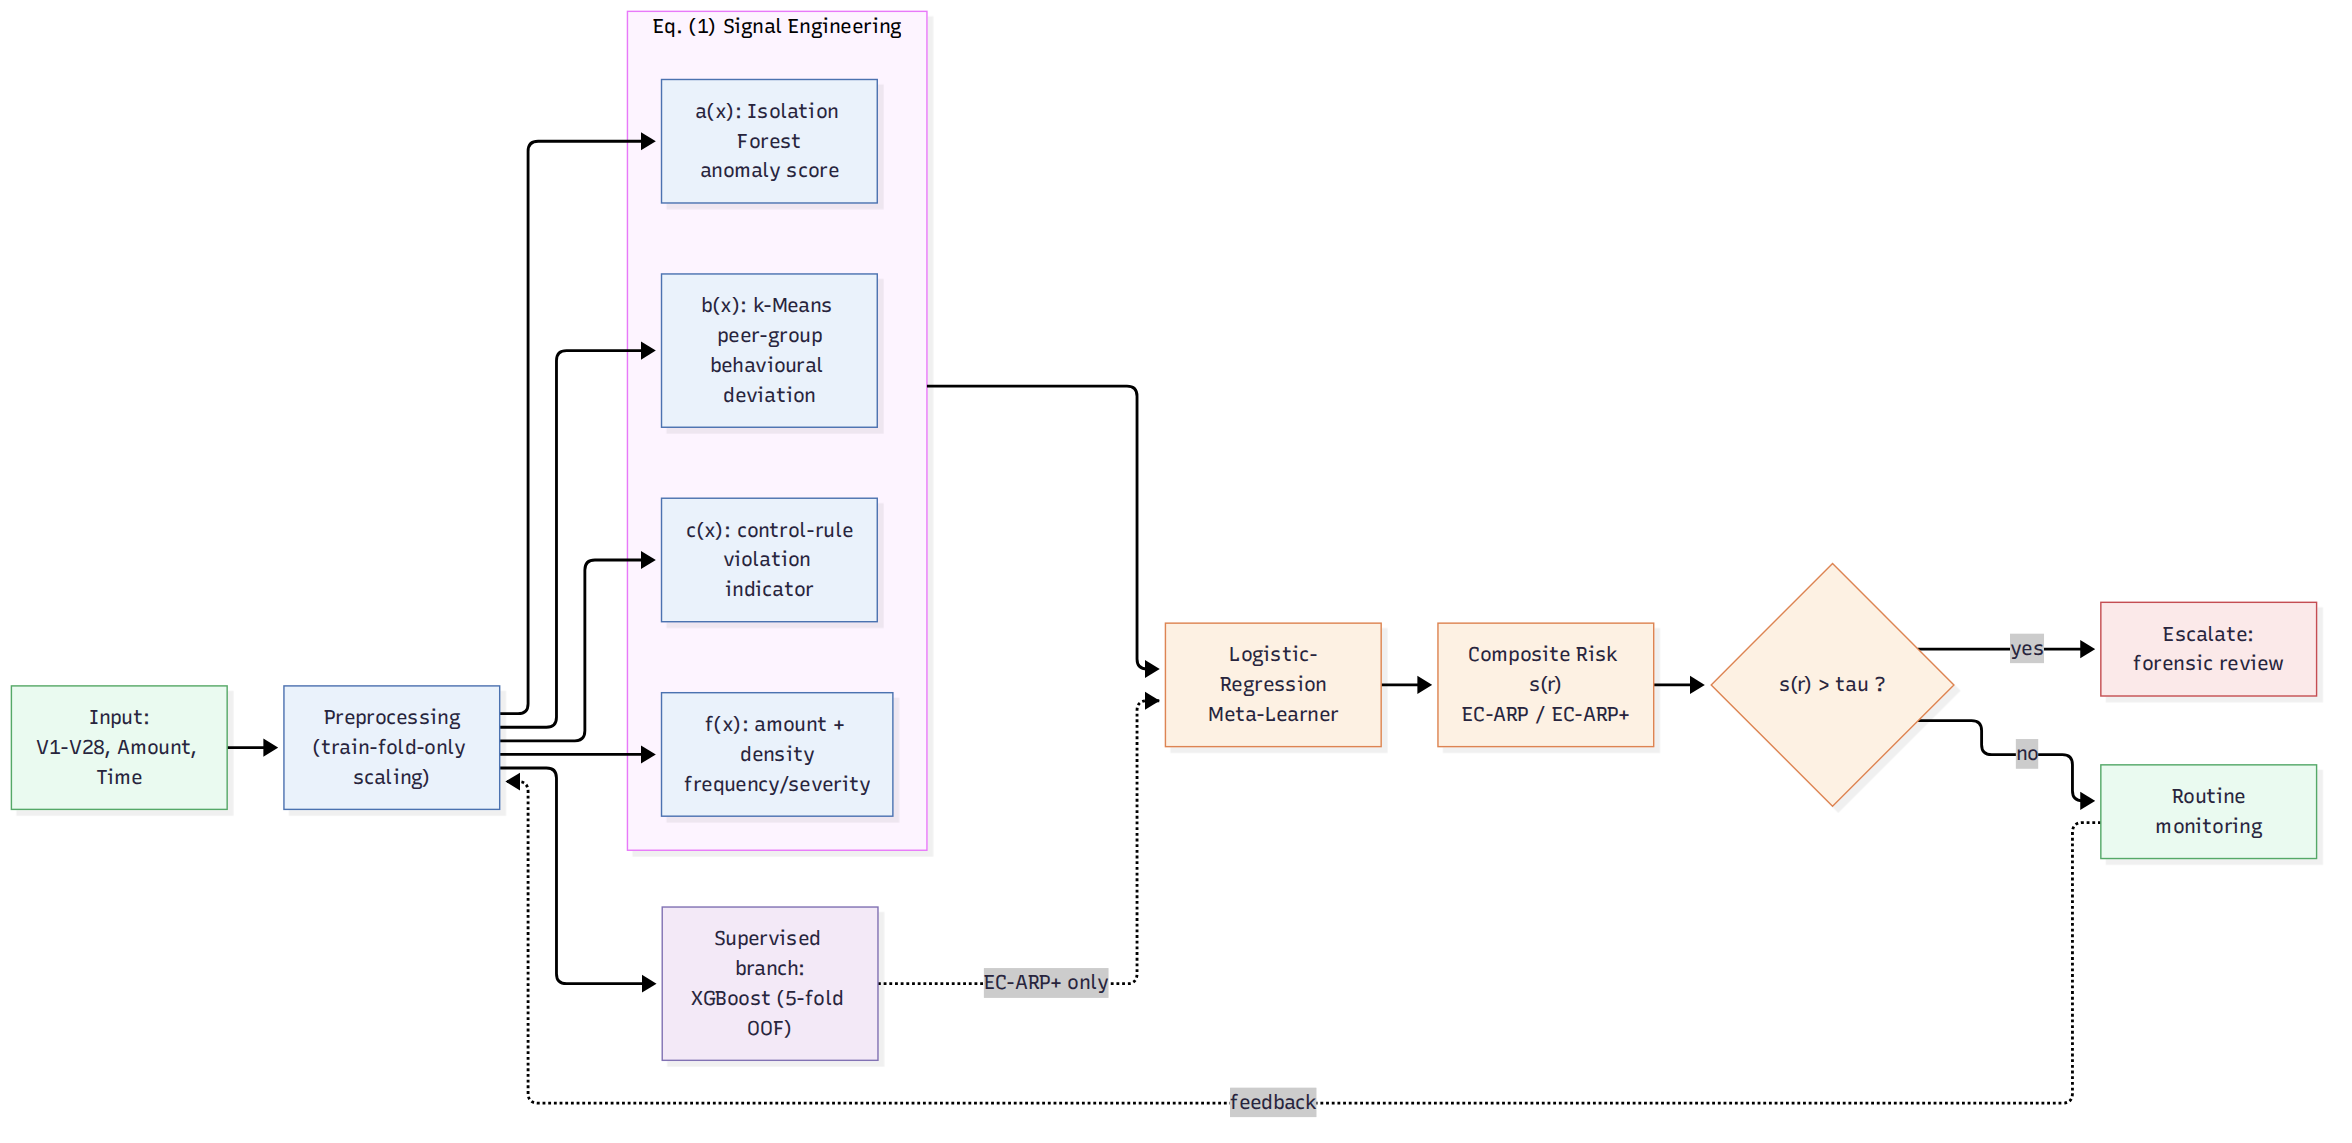
\includegraphics[width=\textwidth]{figs/mermaid_architecture.png}
\caption{Proposed AI-assisted red-flag prioritisation architecture. The four Eq.~\eqref{eq:risk} signals ($a,b,c,f$) are engineered from transaction data; EC-ARP calibrates their weights via a logistic-regression meta-learner; EC-ARP+ additionally stacks a supervised gradient-boosted signal (dotted path). Records with $s(r)>\tau$ are escalated; outcomes feed back to recalibrate the model.}
\label{fig:architecture}
\end{figure*}

\subsection{Empirical Validation Design}
\label{sec:empirical-method}

To test whether Eq.~\eqref{eq:risk} can be operationalised, and how it performs relative to standard techniques, a benchmark validation study was conducted and released as open, reproducible code.

\subsubsection{Dataset}

The validation uses the ``Credit Card Fraud Detection'' dataset assembled by the Machine Learning Group at Universit\'e Libre de Bruxelles (ULB) in collaboration with Worldline \citep{dalpozzolo2015}. The dataset contains 284,807 transactions made by European cardholders over two days in September 2013, of which 492 (0.173\%) are confirmed fraudulent -- an imbalance ratio of approximately 578:1. Twenty-eight of the 30 predictor features (V1--V28) are principal components of the original transaction attributes, released in anonymised form for confidentiality; the remaining two are \emph{Time} (seconds elapsed since the first transaction) and \emph{Amount} (transaction value). This dataset was selected because it is the most widely used public benchmark for transaction-level fraud detection and therefore supports independent verification of the results, not because it is a substitute for primary audit-log or general-ledger data -- a distinction discussed further in Section~\ref{sec:limitations}. Table~\ref{tab:dataset} summarises the dataset's operational characteristics.

\begin{table}[!t]
\caption{Operational characteristics of the validation dataset}
\label{tab:dataset}
\centering
\footnotesize
\begin{tabular}{ll}
\toprule
\textbf{Description} & \textbf{Details} \\
\midrule
Source & ULB Machine Learning Group / Worldline \citep{dalpozzolo2015} \\
Number of transactions & 284,807 \\
Number of features & 30 (V1--V28 PCA components, Amount, Time) \\
Target variable & Class (0 = legitimate, 1 = fraud) \\
Fraud cases & 492 (0.173\%) \\
Imbalance ratio & 577.9 : 1 (legitimate : fraud) \\
Missing values & 0 \\
Duplicate rows & 1,081 (retained, standard for this benchmark) \\
Amount (mean / median / max) & \$88.35 / \$22.00 / \$25,691.16 \\
\bottomrule
\end{tabular}
\end{table}

\subsubsection{Exploratory Data Analysis}
\label{sec:eda}

Before feature engineering, the dataset was examined descriptively. Figure~\ref{fig:eda-class} shows the class imbalance on a logarithmic scale; Figure~\ref{fig:eda-amount} shows the transaction-amount distribution by class; and Figure~\ref{fig:eda-hour} shows the fraud rate by hour of the relative 24-hour transaction clock derived from the \emph{Time} field, which is visibly non-uniform, with fraud rates peaking sharply around hours 2 and 4 (1.7\% and 1.0\% respectively, compared with a dataset-wide average of 0.173\%) -- an observation that partially motivated the off-hours component of the control-rule signal $c(x_r)$ in Section~\ref{sec:empirical-method}.

\begin{figure}[!t]
\centering
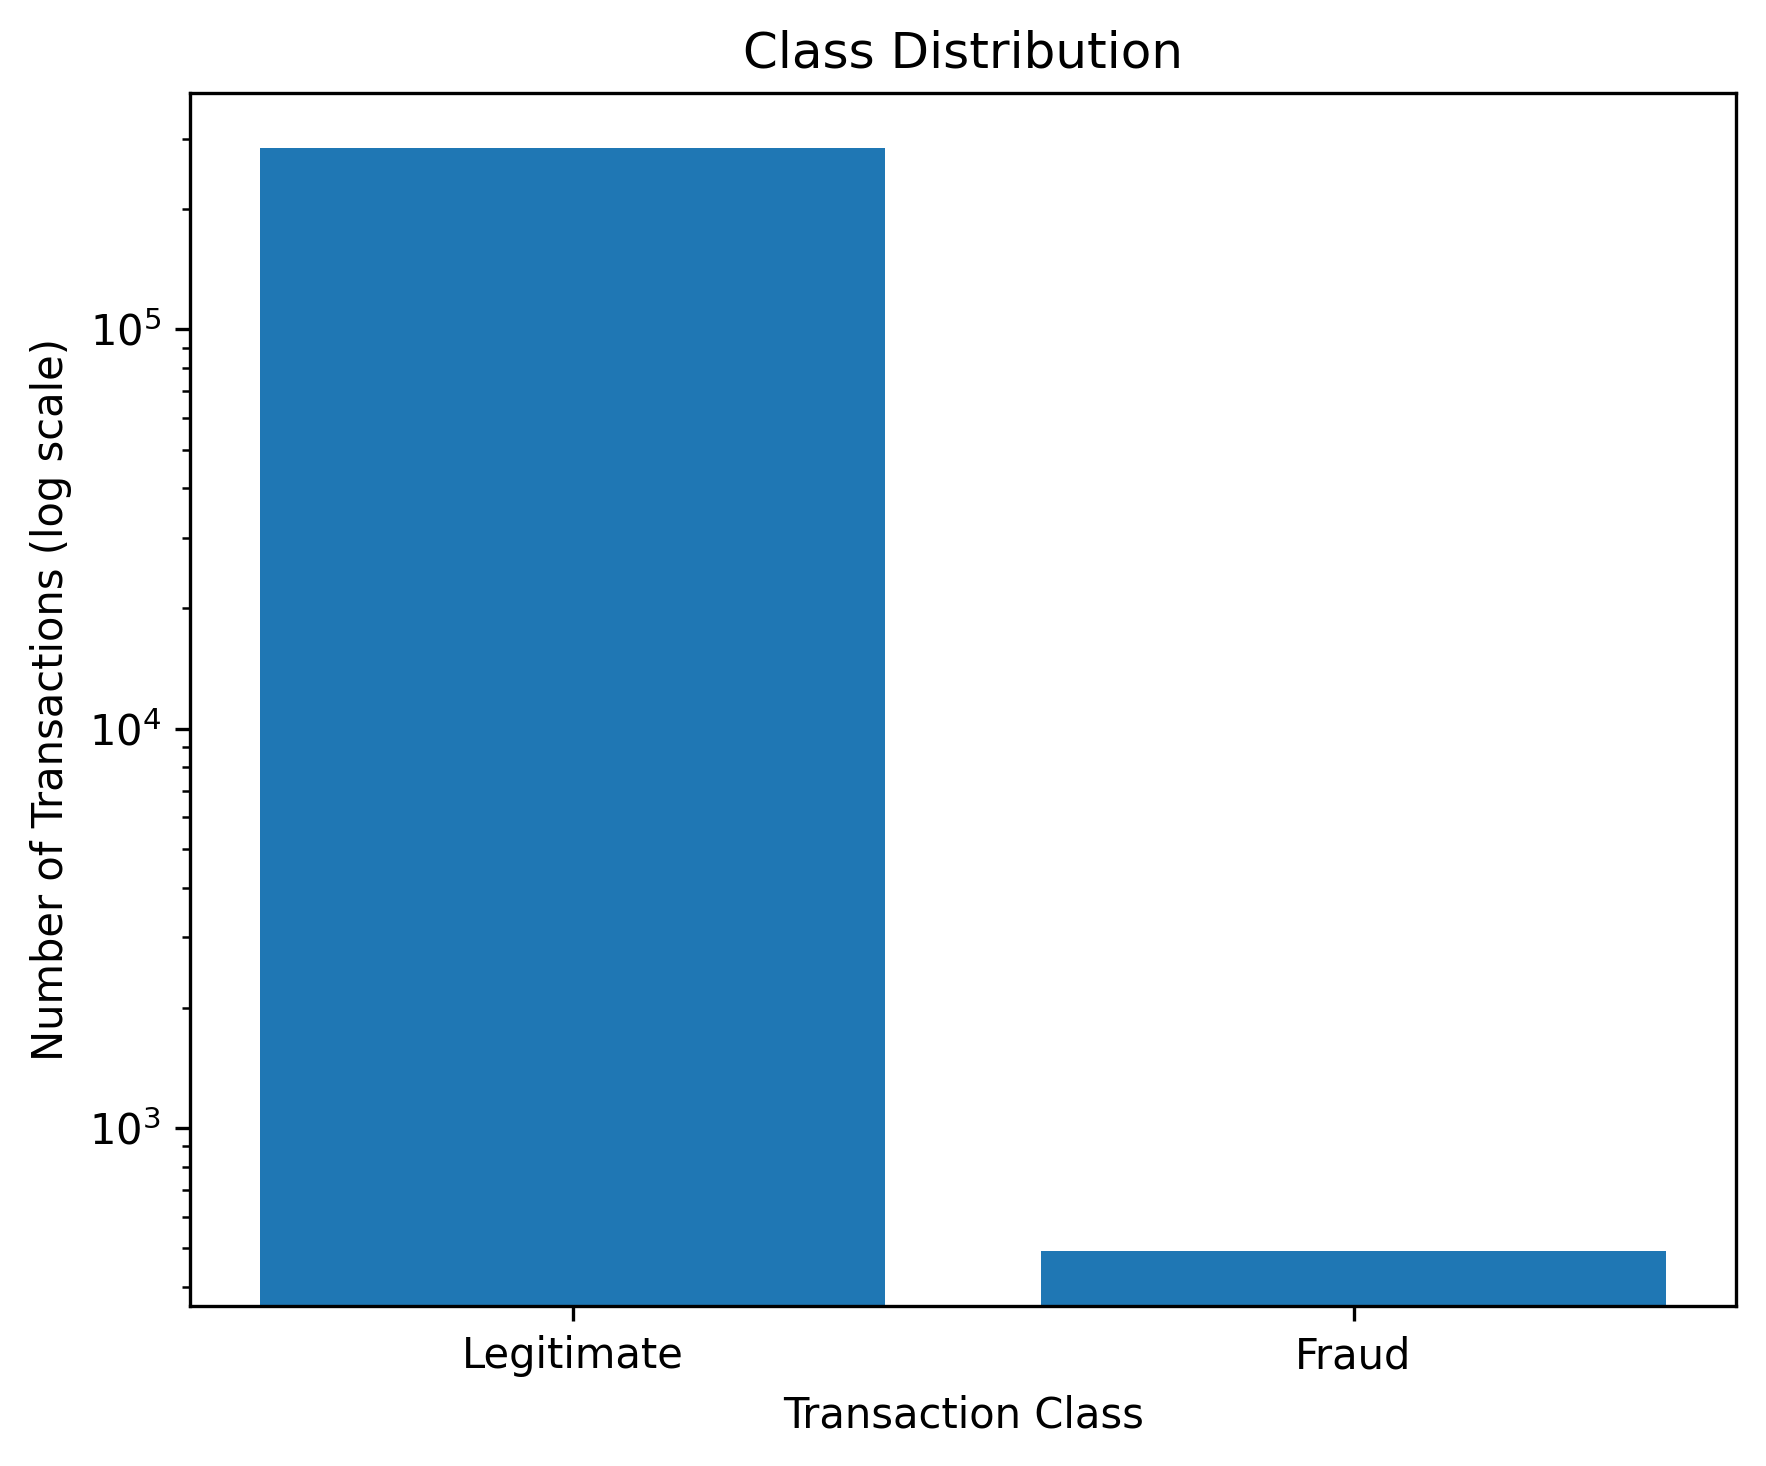
\includegraphics[width=0.9\columnwidth]{figs/eda_class_balance.png}
\caption{Class balance in the validation dataset (log scale): 284,315 legitimate vs.\ 492 fraudulent transactions (0.173\%).}
\label{fig:eda-class}
\end{figure}

\begin{figure}[!t]
\centering
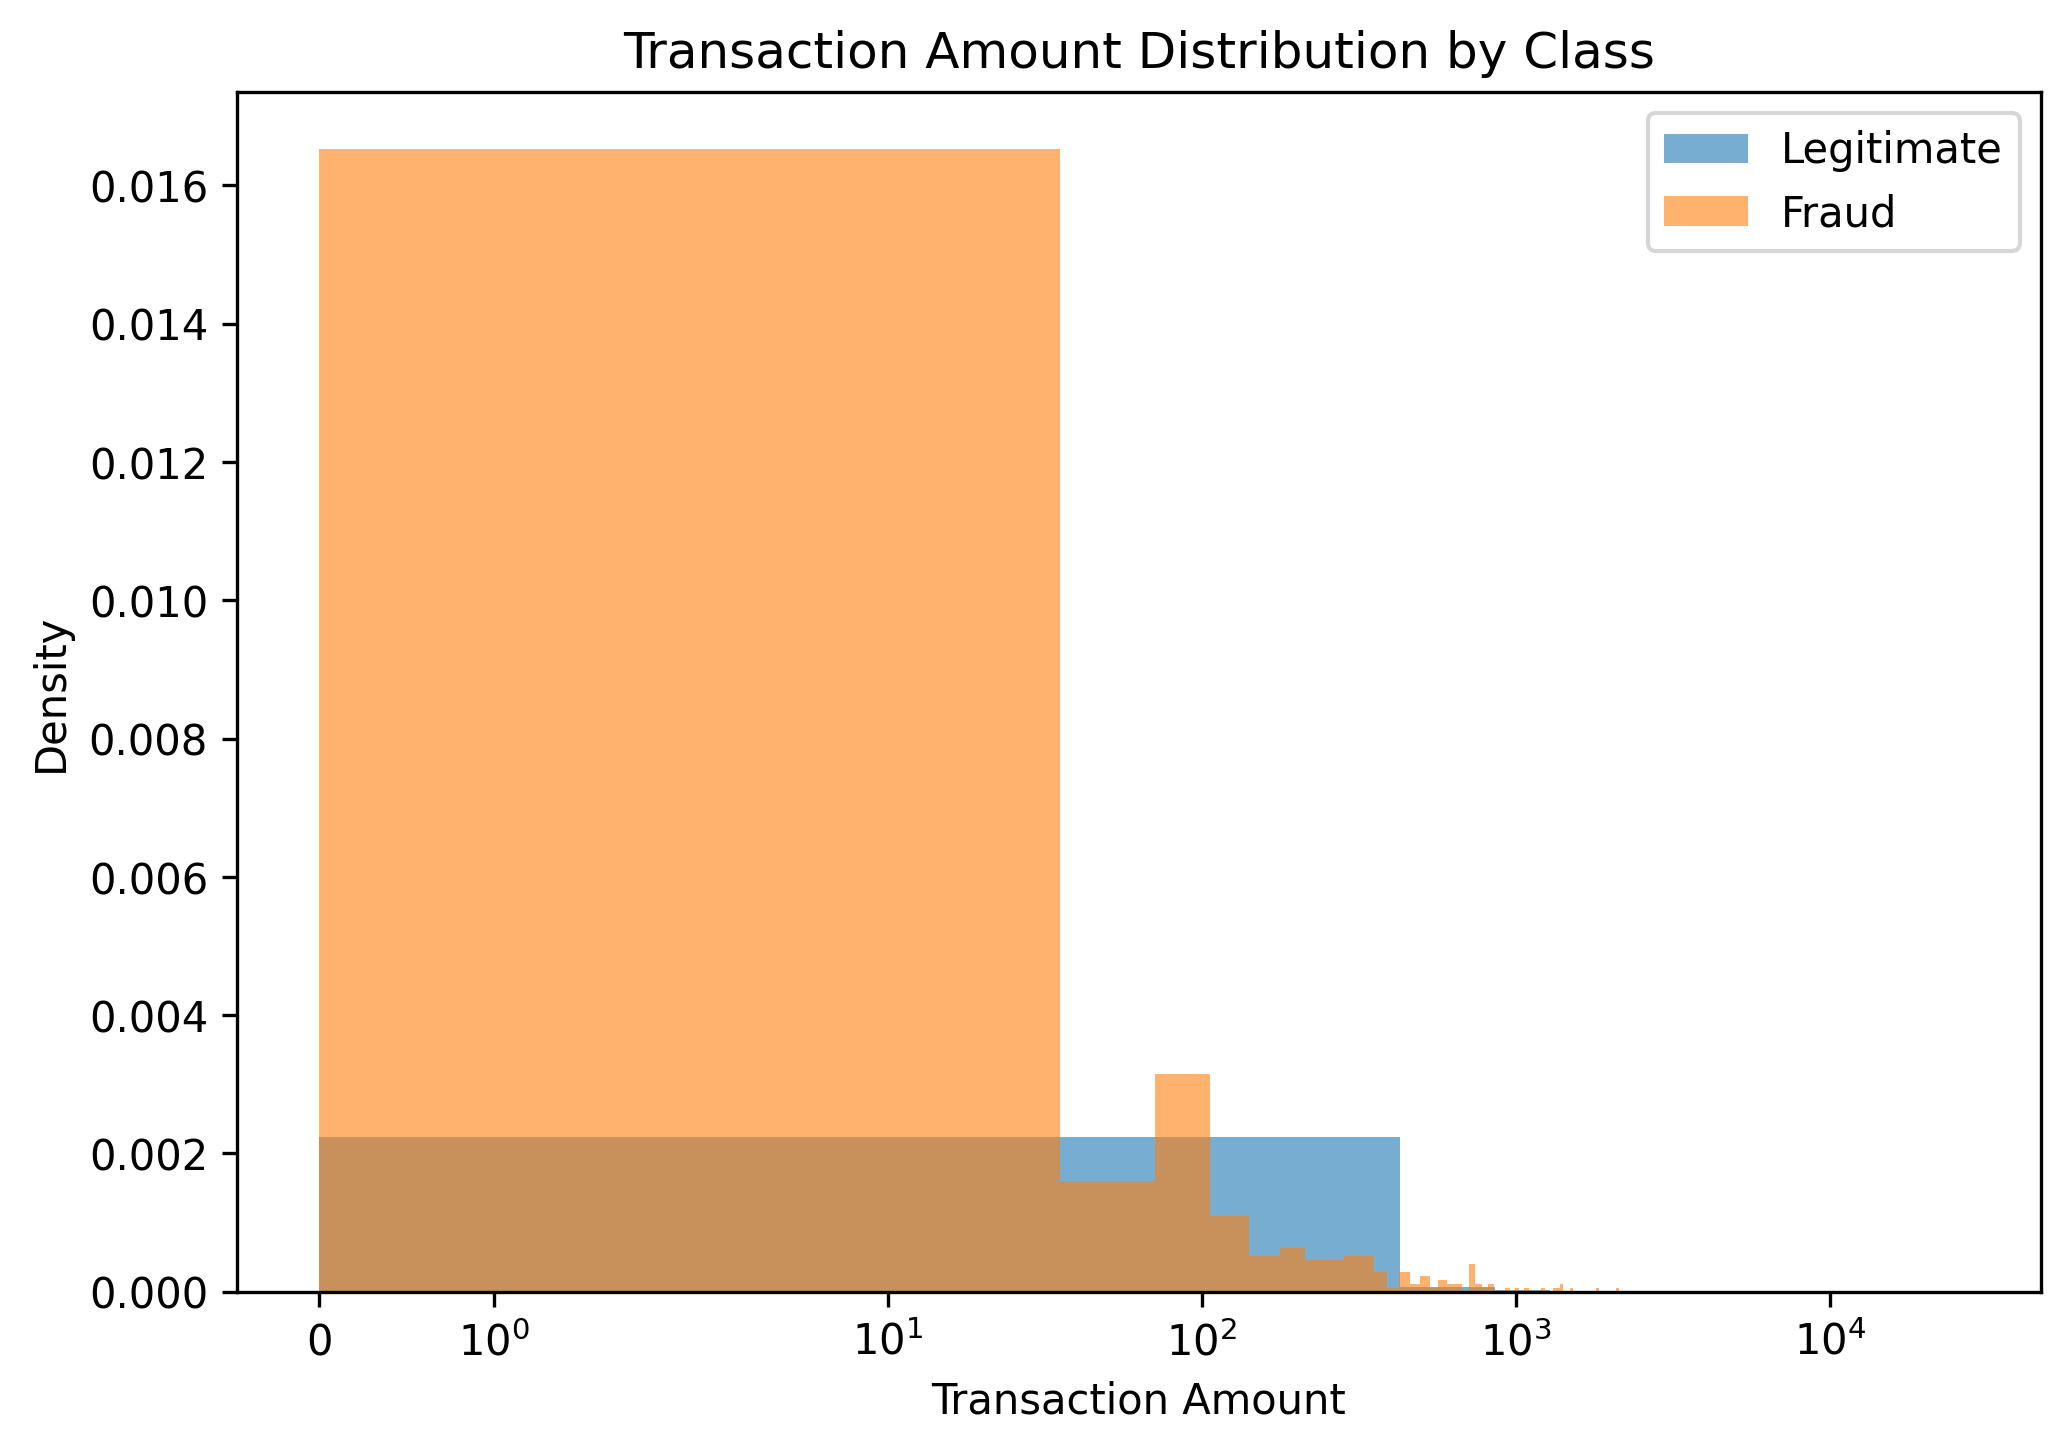
\includegraphics[width=0.9\columnwidth]{figs/eda_amount_distribution.png}
\caption{Transaction amount distribution by class (symmetric log scale).}
\label{fig:eda-amount}
\end{figure}

\begin{figure}[!t]
\centering
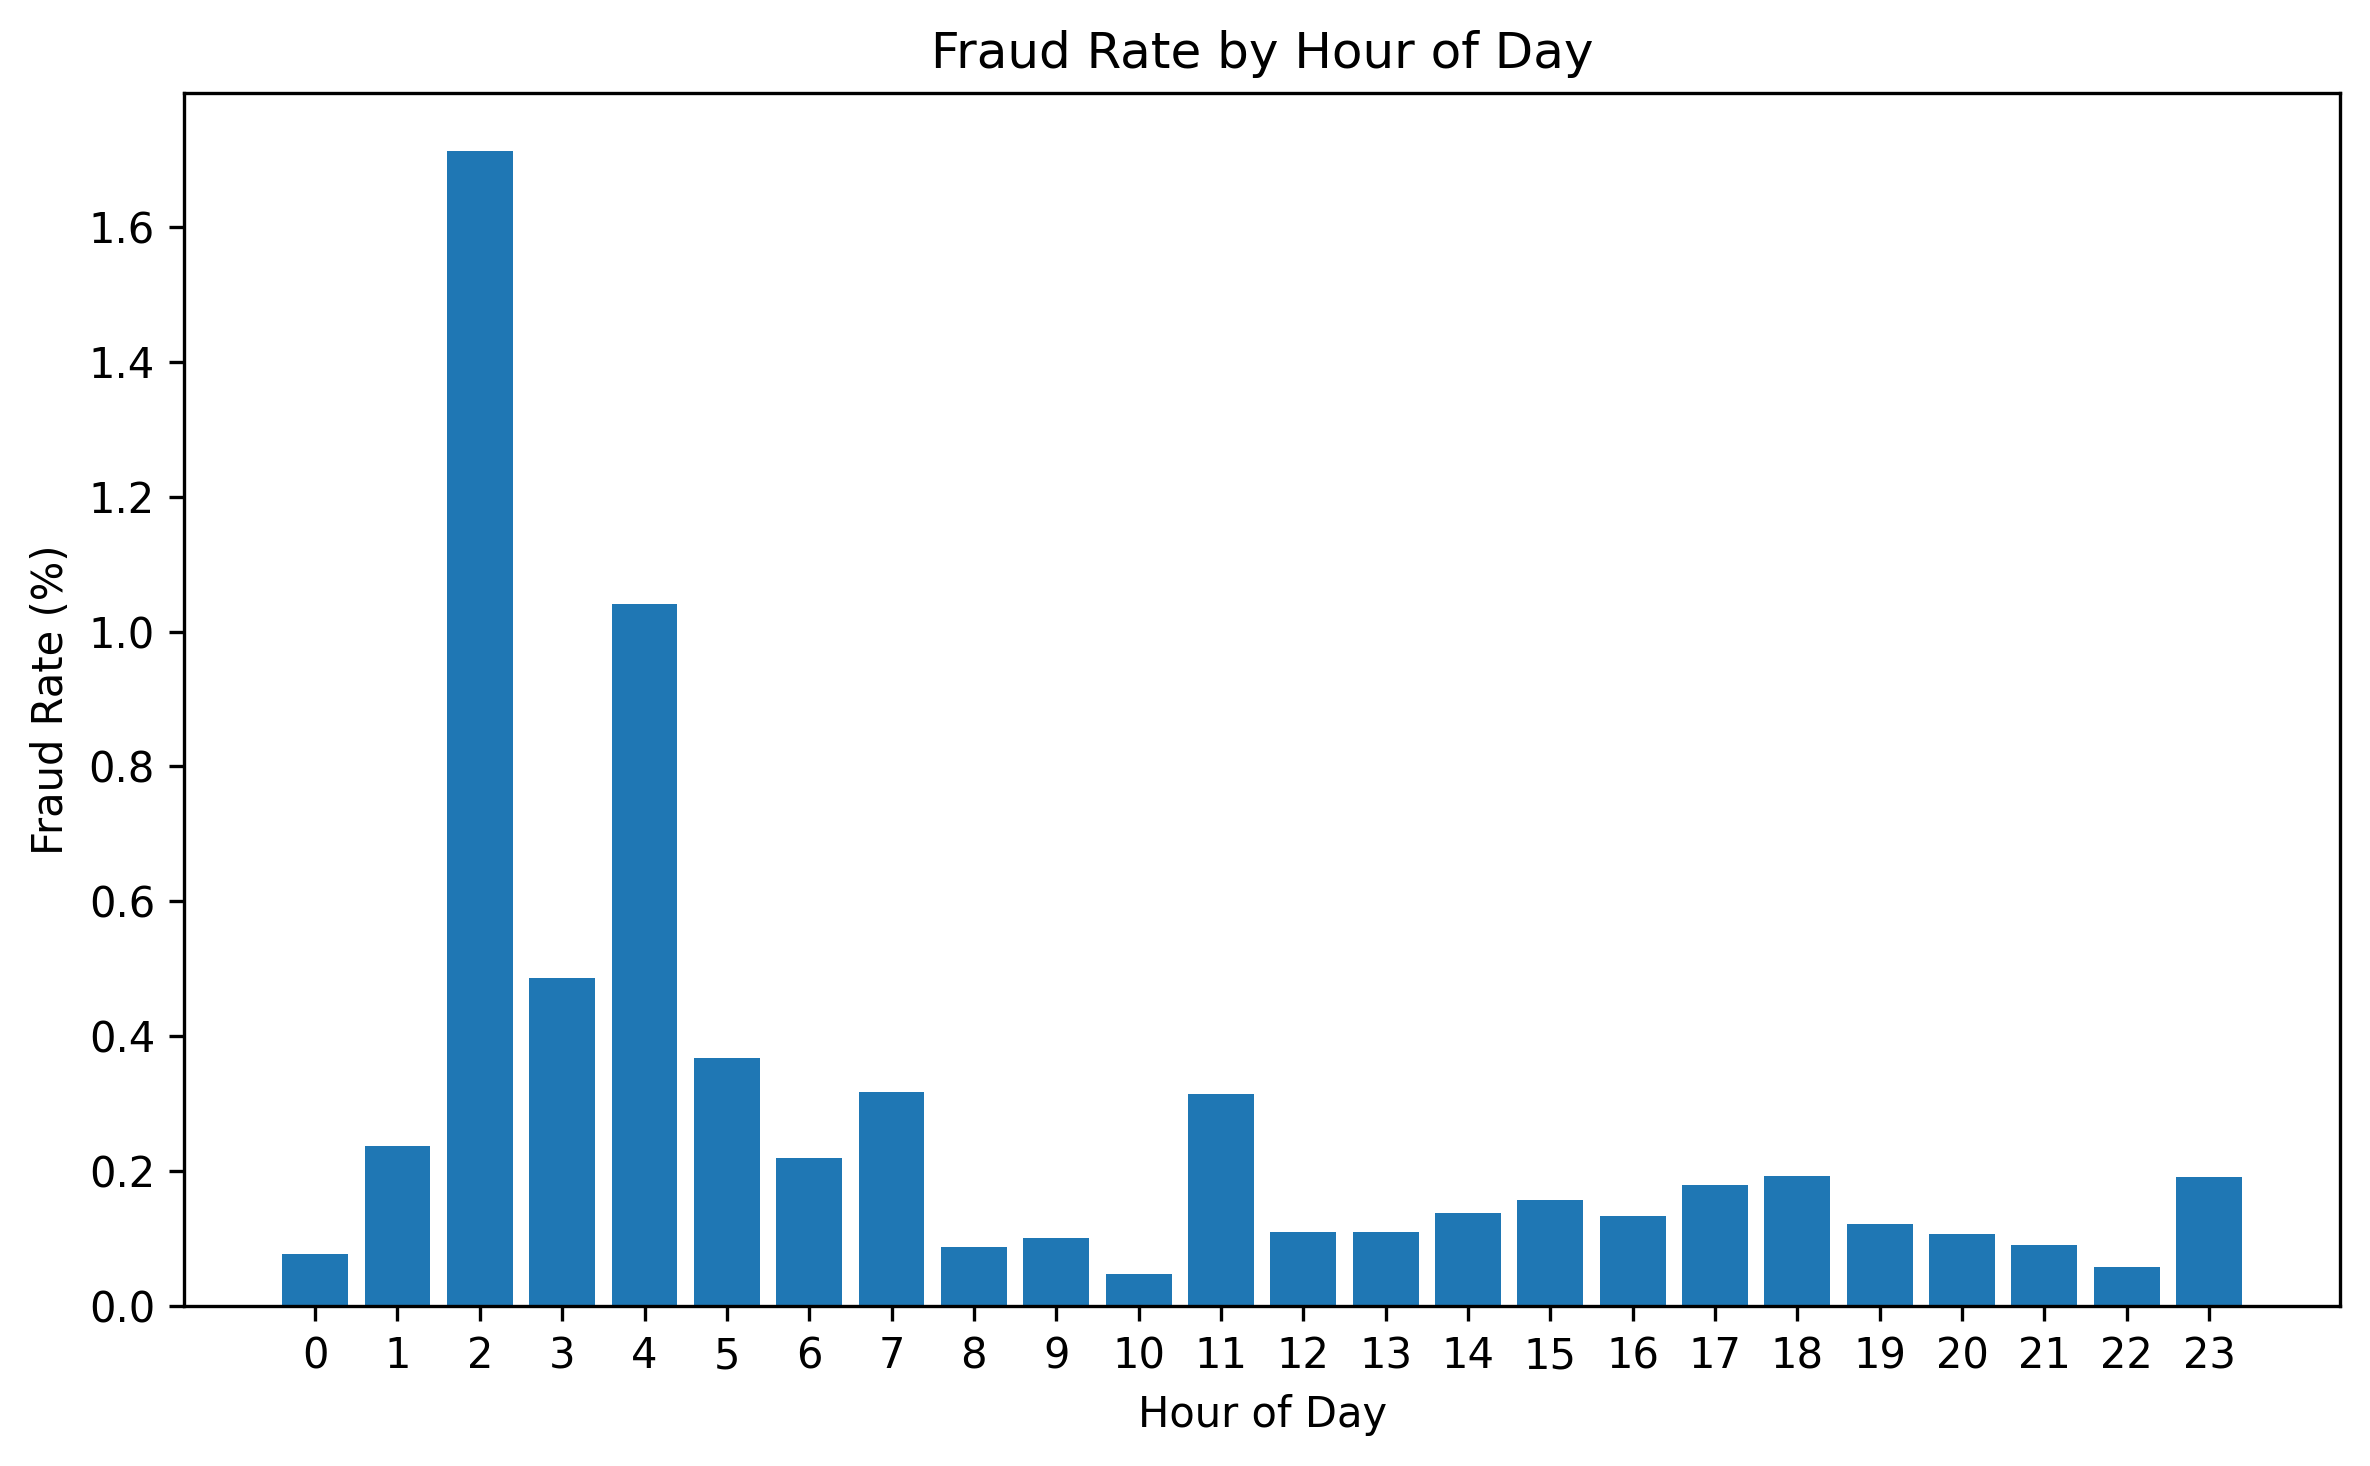
\includegraphics[width=0.9\columnwidth]{figs/eda_fraud_rate_by_hour.png}
\caption{Fraud rate by hour of the relative 24-hour transaction clock, derived from the \emph{Time} field.}
\label{fig:eda-hour}
\end{figure}

Correlation of the anonymised V1--V28 features with the fraud label was also examined (Figures~\ref{fig:eda-corr-top10} and \ref{fig:eda-corr-all}). The strongest associations are negative: V17, V14 and V12 show the largest-magnitude negative correlations with fraud (approximately $-0.33$, $-0.30$ and $-0.26$ respectively), followed by V10, V16, V3 and V7 (all between approximately $-0.19$ and $-0.22$). The strongest positive associations are V11 and V4 (approximately $+0.15$ and $+0.13$). Because V1--V28 are principal components of the original, undisclosed transaction attributes, these correlations indicate which latent dimensions are most discriminative but cannot be mapped back to concrete business variables -- a limitation of this benchmark noted again in Section~\ref{sec:limitations}. The isolation-forest and $k$-means signals used for $a(x_r)$ and $b(x_r)$ operate on the full standardised V1--V28 space and therefore implicitly draw on all of these correlated dimensions rather than on any single feature.

\begin{figure}[!t]
\centering
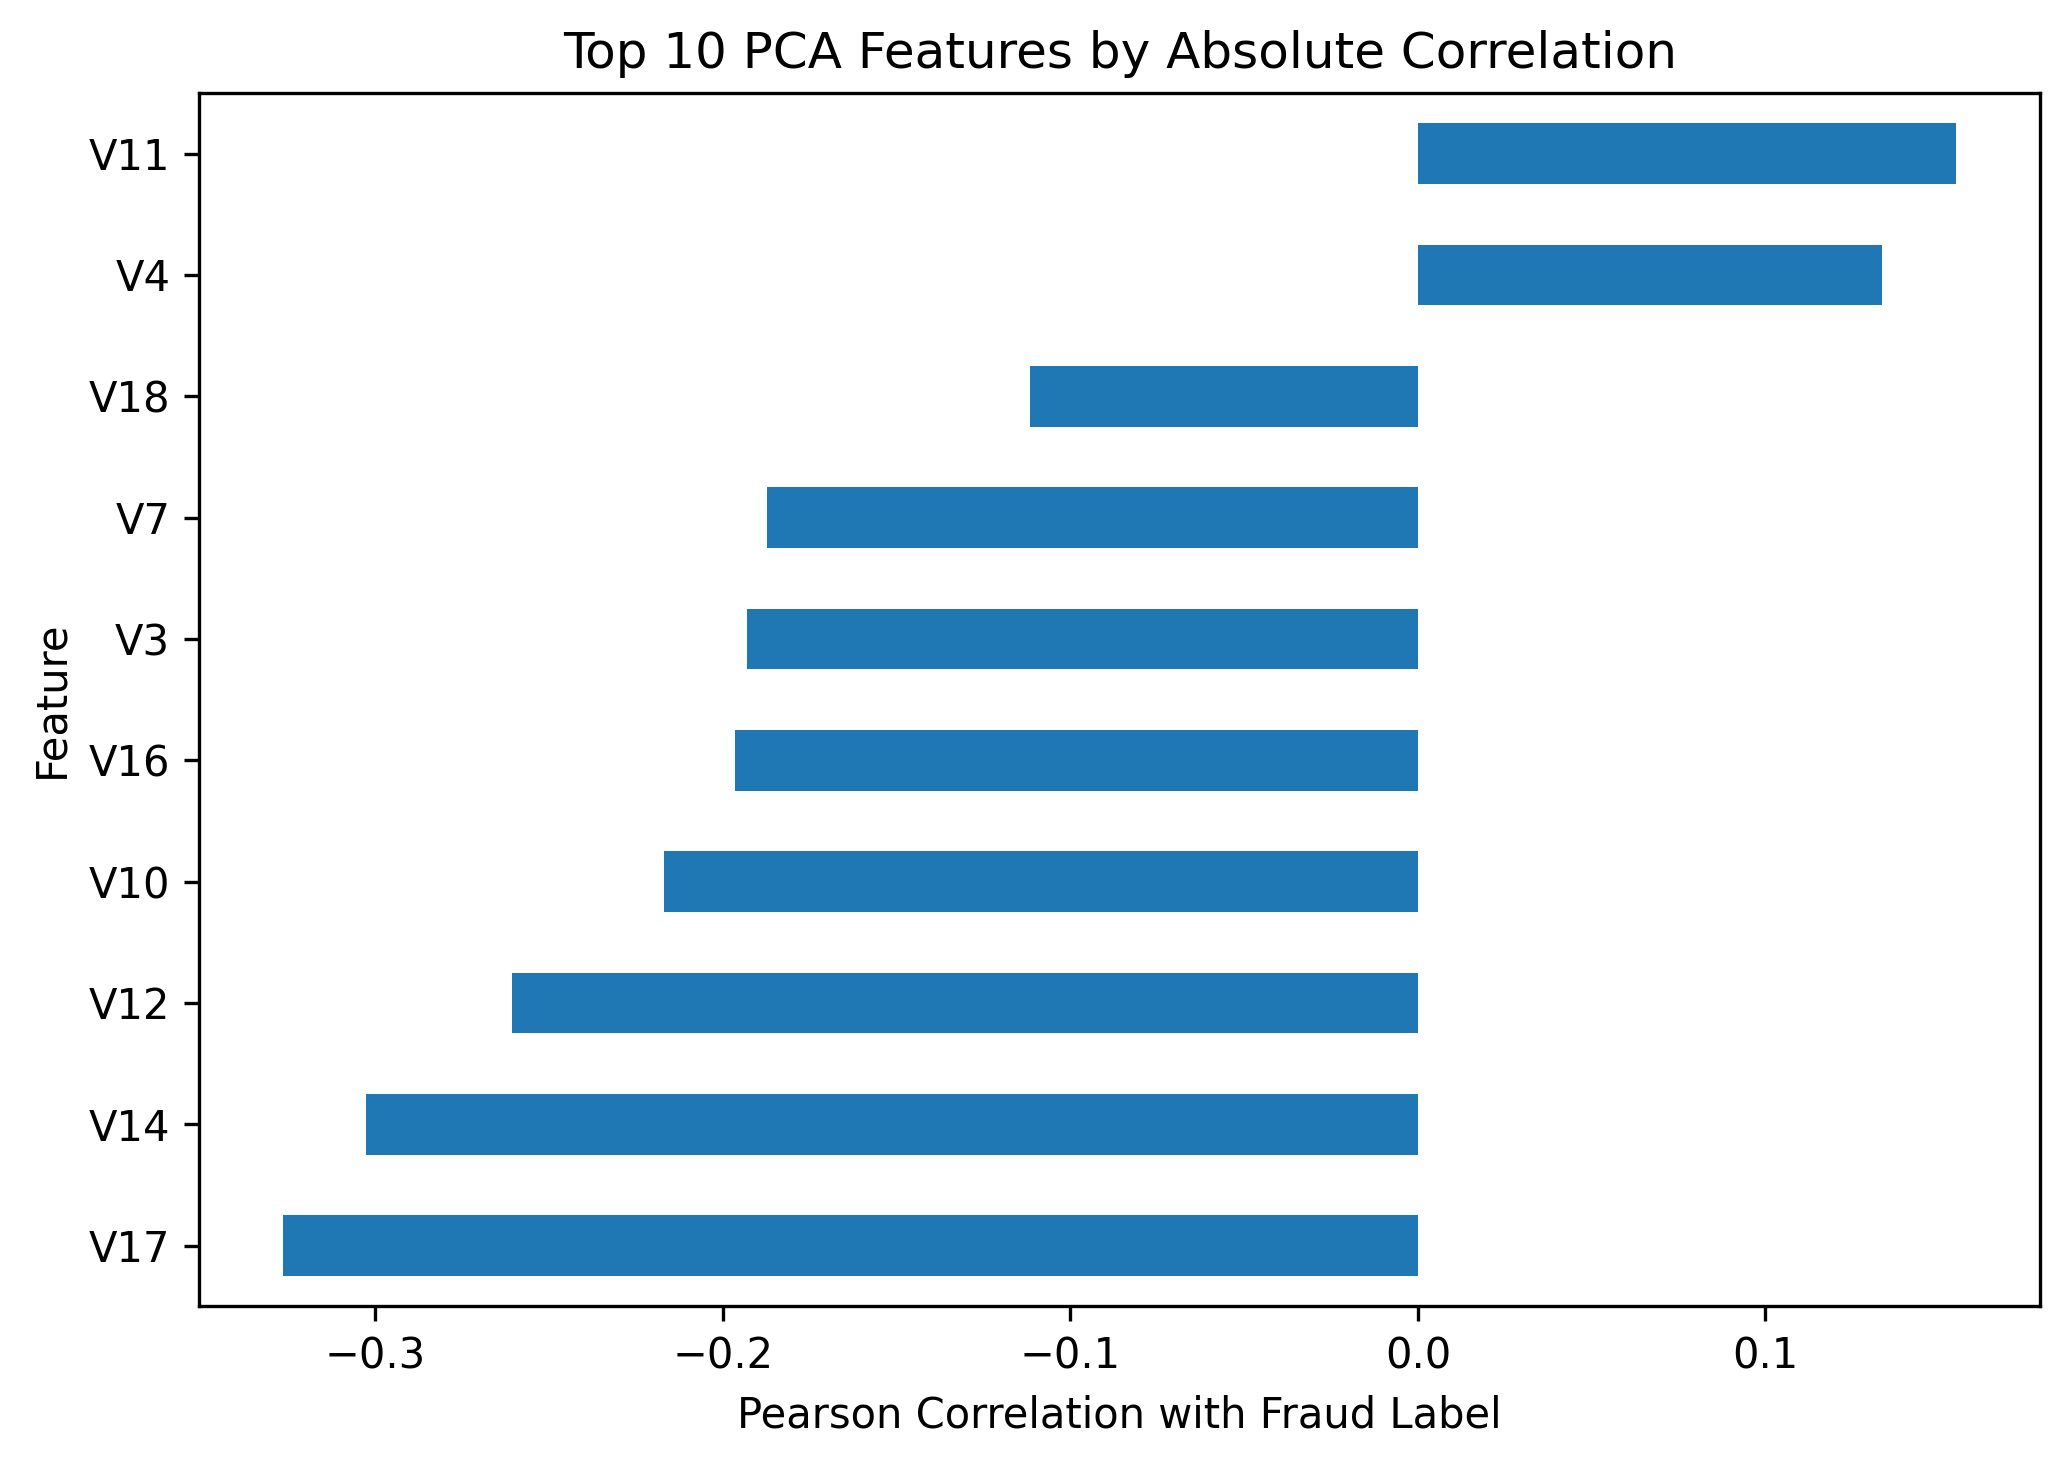
\includegraphics[width=0.9\columnwidth]{figs/eda_feature_correlation_top10.png}
\caption{Top 10 V1--V28 features by absolute Pearson correlation with the fraud label.}
\label{fig:eda-corr-top10}
\end{figure}

\begin{figure}[!t]
\centering
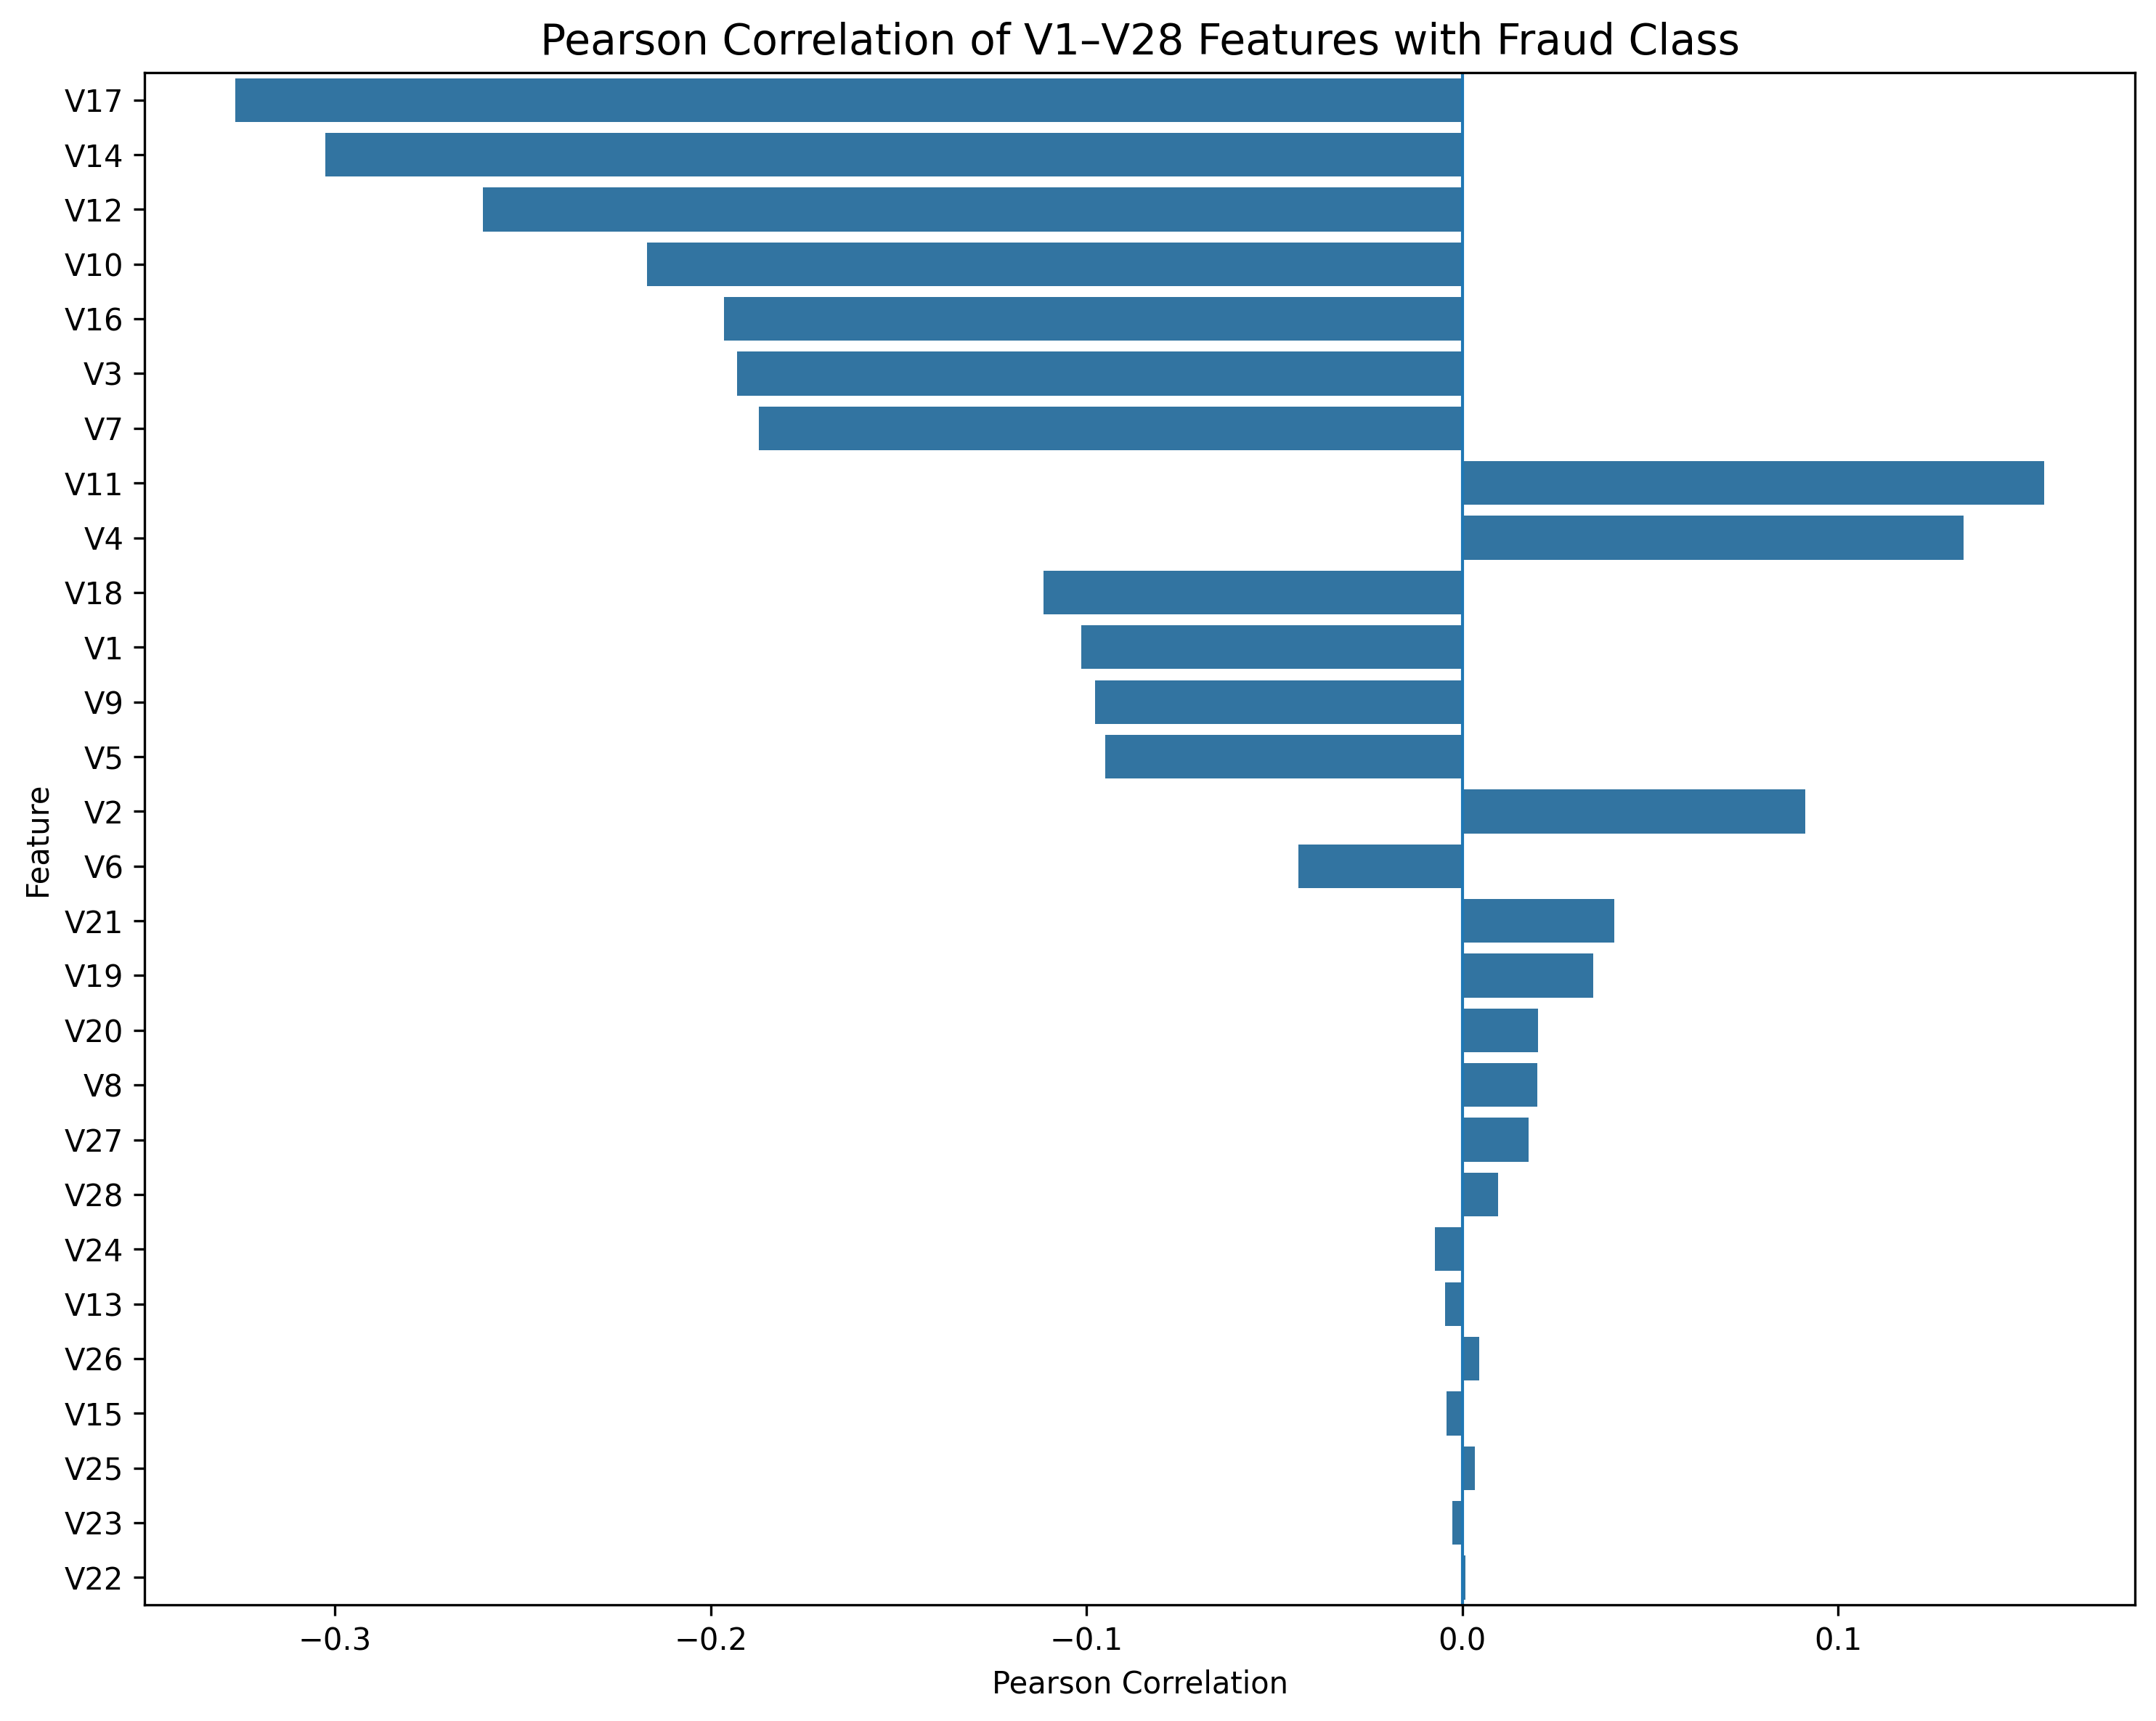
\includegraphics[width=0.9\columnwidth]{figs/eda_feature_class_correlation.png}
\caption{Pearson correlation of all 28 V1--V28 features with the fraud label.}
\label{fig:eda-corr-all}
\end{figure}

\subsubsection{Operationalising Eq.~\eqref{eq:risk}}

Each term of Eq.~\eqref{eq:risk} is computed as follows, fitted only on a training partition to avoid information leakage into the held-out test set:
\begin{itemize}
    \item $a(x_r)$ -- an isolation-forest anomaly score \citep{liu2008} computed on the standardised V1--V28 features, min-max scaled to $[0,1]$;
    \item $b(x_r)$ -- a behavioural-deviation score computed as the Euclidean distance from each transaction to its nearest centroid under a 12-cluster MiniBatch $k$-means peer-group clustering of the standardised V1--V28 features, min-max scaled to $[0,1]$;
    \item $c(x_r)$ -- a binary control-rule indicator equal to 1 if the transaction amount exceeds the 99th percentile of training-set amounts \emph{or} the transaction occurs in the first five hours of its relative 24-hour clock cycle (an off-hours proxy derived from the \emph{Time} field), and 0 otherwise;
    \item $f(x_r)$ -- an equally weighted combination of normalised transaction amount (severity) and local transaction density within a $\pm$60-second window (a frequency/burst proxy), each min-max scaled to $[0,1]$.
\end{itemize}
A principal-component reconstruction-error term is computed separately (10-component PCA fitted on the training partition; mean squared reconstruction error on the standardised V1--V28 features) and used only as a standalone \emph{baseline} anomaly detector, standing in for an autoencoder given that V1--V28 are themselves already PCA outputs.

\subsubsection{Proposed models and baselines}

Two instantiations of Eq.~\eqref{eq:risk} are evaluated. \textbf{EC-ARP} (Empirically-Calibrated AI-assisted Red-flag Prioritisation) is a logistic-regression meta-learner trained on $[a(x_r), b(x_r), c(x_r), f(x_r)]$, with coefficients clipped to be non-negative and re-normalised to sum to one, giving weights $w_1$--$w_4$ that satisfy the constraints of Eq.~\eqref{eq:risk} while being fitted rather than assumed. \textbf{EC-ARP+} extends this with a fifth input -- an out-of-fold XGBoost \citep{chen2016} probability obtained via 5-fold cross-validation on the training partition -- yielding a fifth calibrated weight $w_5$ (Figure~\ref{fig:architecture}). Four baselines mirror techniques reported individually in the reviewed literature: logistic regression with class-balanced weighting; a random forest \citep{breiman2001} (300 trees, class-balanced subsampling); XGBoost \citep{chen2016} (400 trees, learning rate 0.05, positive-class weighting); and the isolation-forest \citep{liu2008} anomaly score $a(x_r)$ used alone. The PCA reconstruction-error detector is included as a fifth, purely unsupervised baseline.

\subsubsection{Evaluation protocol}

Data were split once into a stratified 70\%/30\% train/test partition (train $n=199{,}364$; test $n=85{,}443$; \texttt{random\_state}=42), preserving the 0.173\% fraud rate in both partitions. All unsupervised components (isolation forest, $k$-means, PCA) and all supervised models are fitted only on the training partition. Given the severe class imbalance, the area under the precision--recall curve (PR-AUC / average precision) is reported as the primary metric, alongside ROC-AUC, F1/precision/recall at a 0.5 probability threshold, and precision/recall at the top 1\% of transactions ranked by score -- the last of these operationalising the threshold $\tau$ in Eq.~\eqref{eq:risk} as a fixed audit-investigation capacity constraint, the metric considered most relevant to practice.

\section{Results and Discussion}
\label{sec:results}

This section synthesises the reviewed evidence around RQ1--RQ4 and then reports the empirical validation results for RQ5.

\subsection{Analytical Maturity and Fraud Detection Efficacy}
\label{sec:maturity}

The value of business analytics in auditing is strongly influenced by the maturity of the analytical technologies and models applied. Organisations that progress from fundamental descriptive techniques to advanced prescriptive analytics generally achieve substantial gains in fraud-detection accuracy \citep{lokanan2024}. Descriptive analytics analyses key patterns and historical trends; diagnostic analytics assesses the underlying causes of anomalies; predictive analytics anticipates potential misconduct before its occurrence; and prescriptive analytics uses higher-level algorithms, including artificial intelligence and machine learning, to recommend the best actions in real time \citep{pamisetty2021}. The reviewed sources report a substantial increase in fraud-detection success across this maturity span: descriptive analytics is reported to achieve markedly lower anomaly-detection rates because of its passive character \citep{yv2021}, while predictive and prescriptive techniques are reported to achieve substantially higher accuracy when trained on well-curated data and calibrated against fraud taxonomies \citep{machireddy2022}. This advancement is not without obstacles: transitioning to advanced analytics requires infrastructure investment, skilled personnel and effective change management, and organisations in diagnostic or early predictive stages often struggle to justify and validate the investment required for prescriptive systems \citep{malempati2025}. Analytics maturity therefore couples technological infrastructure with cultural adaptability and long-term strategic orientation.

\subsection{Tool-Specific Outcomes and Practical Applications}

An in-depth evaluation of prominent audit-analytics platforms -- ACL, IDEA, Power BI, Tableau and Python -- shows specific advantages and disadvantages regarding detection precision, usability and system compatibility. Open-source technologies such as Python and R provide advanced analytical functions and demonstrate effectiveness in simulating fraudulent scenarios and detecting anomalies \citep{eldahshan2024}; these techniques are reported to be highly applicable in high-risk industries such as finance and e-commerce, where fraudulent practices frequently advance beyond the detection capabilities of conventional rule-based approaches \citep{balogun2021}. Tableau and Power BI, by contrast, excel in environments emphasising visual exploration and presentation of financial data; although lacking native fraud-detection capabilities, they provide visualisation tools that assist auditors in analysing trends and correlations \citep{thakkar2025}. IDEA is reported to function as a pragmatic intermediary, applied for file-consistency verification, fuzzy-logic comparisons and regression-based anomaly identification, while ACL's limited advanced-detection capability is offset by a user-friendly interface and standardised reporting that render it a reliable choice for structured audit processes \citep{pinto2024}. Effectiveness ultimately depends on an entity's technical proficiency, data quality and the complexity of the fraud threats considered \citep{sewpersadh2025}, and combining different tools is reported to sharpen fraud detection and expedite informed decision-making \citep{javaid2024}.

\subsection{Typological Distribution of Red-Flag Indicators}

The identification and categorisation of red-flag indicators is essential to fraud detection. The typological matrix (Section~\ref{sec:taxonomy}) classifies indicators into five primary categories, drawing on the reviewed literature \citep{aivaz2024}. Transaction irregularities -- often arising from frequent transactions, unusual timing or minor discrepancies -- account for the largest share of detected anomalies and typically reveal flaws in digital systems or approval workflows. Document manipulation, including fake invoices, duplicate records or unapproved changes, is also widespread and points to systemic vulnerabilities in invoice authorisation and documentation integrity \citep{nogueira2025}. Behavioural anomalies are frequently associated with sudden changes in employee conduct, irregular access patterns, or overt resistance to oversight and internal audits, and may be considered early indicators of hidden misconduct \citep{douglas2024}. Structural discrepancies arise from inconsistencies across financial statements, business units or reporting structures, often pointing to isolated internal-control systems and governance gaps \citep{qatawneh2024}. Relational fraud is less prevalent and considerably more elusive, requiring advanced techniques -- such as graph-based analytics and cross-entity tracking -- to detect schemes like bid-rigging or collusive networks \citep{hilal2022}; as such schemes normally evade rule-based detection, advanced pattern-recognition and clustering models are essential for identification \citep{popoola2023}.

The impact on auditing methods is significant. Firms require a multi-tiered red-flag detection system supporting dynamic monitoring of financial operations \citep{adejumo2025}, and real-time analytics capturing evolving financial patterns should replace conventional reactive models. Practitioners must also recognise that many fraud signals do not exist independently -- intersecting signals across categories may indicate elevated risk and demand more comprehensive diagnostic models, a consideration reflected directly in the multi-term structure of Eq.~\eqref{eq:risk}. Adopting machine-learning classifiers augmented with domain-specific knowledge is reported to improve the sensitivity and specificity of red-flag detection \citep{baeyaert2025}.

\subsection{Sectoral and Institutional Distinction in Analytical Application}

The practical implementation of audit analytics differs significantly across sectors, influenced by regulatory rigour, risk exposure, technological capability and organisational priorities \citep{bello2024}. In highly regulated sectors such as finance, healthcare and telecommunications, adoption is generally more advanced: these sectors face rigorous compliance mandates and complex operating frameworks that demand real-time monitoring, predictive fraud-detection algorithms and integrated enterprise platforms \citep{sutisna2025}. Adoption remains more limited in lower-resource industries -- manufacturing, retail and small to medium-sized firms often operate with constrained budgets, weaker IT infrastructure and less integrated data systems \citep{akter2025}, leaving them reliant on basic visualisation software or easily implemented commercial tools that frequently lack the analytical depth required for timely detection \citep{ayodeji2024}. The public sector and non-profit institutions present a distinct trajectory: despite limited funding, these entities remain significantly susceptible to procurement irregularities, misappropriation of funds and misuse of donor-restricted assets \citep{pizzini2025}, and analytics adoption in these contexts demands frameworks tailored to lower technical literacy, operational fragmentation and rigorous compliance standards \citep{alexomiogbemi2024}. Institutional readiness, data-governance culture and the alignment of analytical strategy with business objectives collectively shape analytics maturity more than the mere availability of technology \citep{solano2024}.

\subsection{Organisational Readiness and Comparative Capability Gaps}

Successful application of audit analytics depends substantially on institutional readiness and adaptability. Table~\ref{tab:readiness} shows that deficiencies in audit maturity are influenced by tool availability as well as by personnel competencies, systems-integration difficulties and organisational reluctance to change.

\begin{table}[!t]
\caption{Comparative Organisational Readiness Across Audit Models}
\label{tab:readiness}
\centering
\footnotesize
\begin{tabular}{p{0.24\columnwidth} p{0.20\columnwidth} p{0.42\columnwidth}}
\toprule
\textbf{Parameter} & \textbf{Traditional auditing} & \textbf{Analytics-driven auditing} \\
\midrule
Tool adaptability & Low & High \citep{wagener2025} \\
Staff proficiency & High in accounting & Hybrid (accounting + data) \citep{oliveira2022} \\
Data infrastructure & Manual / legacy & Automated / data lake \\
Fraud-detection speed & Delayed & Real-time \citep{naoufal2024} \\
Scalability & Limited & High \citep{okoodion2024} \\
\bottomrule
\end{tabular}
\end{table}

Conventional audits prioritise accounting proficiency but exhibit a deficiency in data literacy, whereas analytics-driven approaches require a combination of finance and data-science expertise; organisations without focused recruitment or training may implement tools but struggle to extract meaningful diagnostic insight. Legacy, isolated infrastructure presents an additional limitation, compromising data integrity and restricting anomaly detection, while integrated platforms with real-time data streams support continuous auditing and fraud simulation. Manual audits operate within the bounds of human capacity, whereas analytics-driven systems offer modularity and scalability, so that expansion across organisational units incurs comparatively little additional resource investment once implemented.

\subsection{Workflow Efficacy and Governance Alignment}

Integrating analytics into the audit lifecycle (Section~\ref{sec:workflow}) accelerates procedural efficiency and strategic responsiveness. Rather than a strict linear progression, the five stages function within a flexible feedback loop, in which insights from later stages enhance and improve earlier processes. Data preparation remains the most demanding stage in terms of time and resource allocation, involving cleaning, normalisation, record consolidation and classification, each of which significantly influences the accuracy and performance of downstream analytical models \citep{joshi2021}; many organisations have begun implementing automation technologies, including robotic process automation and extract-transform-load pipelines, to minimise manual effort while increasing data quality and consistency \citep{vajpayee2023}. The risk-scoring stage plays a vital role in prioritising audit activities: anomalies are evaluated on severity, frequency and potential financial impact, and incidents exceeding defined thresholds are escalated for detailed forensic investigation or submitted to senior management for review \citep{henriques2024}. Effective governance alignment ensures that analytical outputs translate into actionable institutional improvements \citep{carreno2024}: patterns identified during the red-flag phase inform upstream decisions and policy revisions -- for example, consistent indicators of procurement-related irregularities may prompt changes to vendor-selection protocols, contract-approval workflows or oversight mechanisms \citep{sarkola2023}. Integrating governance structures within the analytics framework supports a shift from reactive detection towards anticipatory risk mitigation and system-wide accountability.

\subsection{Validation and Forward Pathways}

Triangulation across academic, professional and forensic sources -- cross-referencing material from Big Four firms, forensic-audit reports and publicly available case analyses -- supports the interpretation that analytical tools improve audit outcomes, though it does not by itself establish causal effects. The trajectory ahead requires confronting several enduring constraints: improving data interoperability across platforms \citep{mai2022}; developing auditor competencies in SQL, Python and AI interpretability \citep{george2022}; and establishing worldwide standards for algorithmic audits and explainable artificial intelligence in assurance \citep{akula2021}. Cross-disciplinary collaboration is essential -- audit teams must work with IT, data-science, legal and compliance functions to create comprehensive fraud-detection solutions -- and real-time simulation environments, or ``fraud sandboxes'', may facilitate the testing of algorithmic models without legal or ethical exposure. Implementing structured feedback mechanisms between auditors and model developers can enhance model validity and mitigate bias over time. The empirical validation reported next (Section~\ref{sec:empirical-results}) is a first, modest step in this direction -- conducted on a public benchmark rather than a fraud sandbox with primary audit data -- and its principal contribution is methodological: it demonstrates a reproducible protocol that can be re-applied to primary audit-log data as such data becomes available to researchers.

\subsection{Empirical Validation of the Prioritisation Framework}
\label{sec:empirical-results}

\subsubsection{Model comparison}

Table~\ref{tab:model-comparison} reports held-out test-set performance for all six models described in Section~\ref{sec:empirical-method}. XGBoost achieves the highest PR-AUC (0.842) and a competitive ROC-AUC (0.973). EC-ARP+ is the second-best model on PR-AUC (0.811) and close on ROC-AUC (0.947), despite using only four engineered signals plus a single supervised probability rather than the full 29-dimensional raw feature set used directly by XGBoost and random forest. Random forest (PR-AUC 0.800) and logistic regression on raw features (PR-AUC 0.704) both perform respectably but below XGBoost and EC-ARP+. The two purely unsupervised baselines -- isolation forest alone (PR-AUC 0.235) and the PCA reconstruction-error detector (PR-AUC 0.103) -- perform markedly worse, consistent with the reviewed literature's characterisation of unsupervised anomaly detection as a useful but comparatively weak signal in isolation.

Critically, EC-ARP -- the literal empirically-calibrated Eq.~\eqref{eq:risk} using only $a$, $b$, $c$ and $f$ with no supervised component -- performs poorly (PR-AUC 0.180), only marginally better than the isolation-forest baseline and far below every model that includes a supervised signal. This is reported candidly rather than omitted: the proposed framework, taken literally and fitted without a supervised term, is \emph{not} competitive with standard supervised baselines on this benchmark.

\begin{table*}[!t]
\caption{Model Comparison on the Held-Out Test Set (30\% stratified split, $n=85{,}443$). Sorted by PR-AUC.}
\label{tab:model-comparison}
\centering
\scriptsize
\setlength{\tabcolsep}{4pt}
\resizebox{\textwidth}{!}{%
\begin{tabular}{l c c c c c c c}
\toprule
\textbf{Model} & \textbf{ROC-AUC} & \textbf{PR-AUC} & \textbf{F1@0.5} & \textbf{Precision@0.5} & \textbf{Recall@0.5} & \textbf{Precision@top1\%} & \textbf{Recall@top1\%} \\
\midrule
XGBoost (raw features) & 0.973 & \textbf{0.842} & 0.848 & 0.889 & 0.811 & 0.150 & 0.865 \\
EC-ARP+ (proposed: stacked hybrid) & 0.947 & 0.811 & 0.218 & 0.125 & 0.845 & 0.146 & 0.845 \\
Random Forest (raw features) & 0.977 & 0.800 & 0.803 & 0.873 & 0.743 & 0.147 & 0.851 \\
Logistic Regression (raw features) & 0.970 & 0.704 & 0.119 & 0.064 & 0.872 & 0.147 & 0.851 \\
Isolation Forest alone ($a$ only) & 0.943 & 0.235 & -- & -- & -- & 0.104 & 0.601 \\
EC-ARP (proposed: calibrated Eq.~\eqref{eq:risk}) & 0.942 & 0.180 & 0.050 & 0.026 & 0.824 & 0.108 & 0.622 \\
PCA reconstruction error (autoencoder proxy) & 0.934 & 0.103 & -- & -- & -- & 0.088 & 0.507 \\
\bottomrule
\end{tabular}%
}
\end{table*}

At the operationally relevant top-1\% investigation-capacity threshold -- an auditor able to review only the top 855 of 85,443 ranked transactions -- the four supervised-informed models converge to similar performance: recall between 0.845 (EC-ARP+) and 0.865 (XGBoost), and precision between 0.146 and 0.150. This convergence suggests that once a supervised signal is present, the specific choice among XGBoost, random forest, logistic regression and EC-ARP+ matters comparatively little for a fixed audit-triage capacity, whereas the presence or absence of a supervised signal matters a great deal (compare EC-ARP+'s 0.845 recall at top 1\% against EC-ARP's 0.622 and isolation forest's 0.601). Figures~\ref{fig:pr-curves} and \ref{fig:roc-curves} present the full precision--recall and ROC curves.

\begin{figure}[!t]
\centering
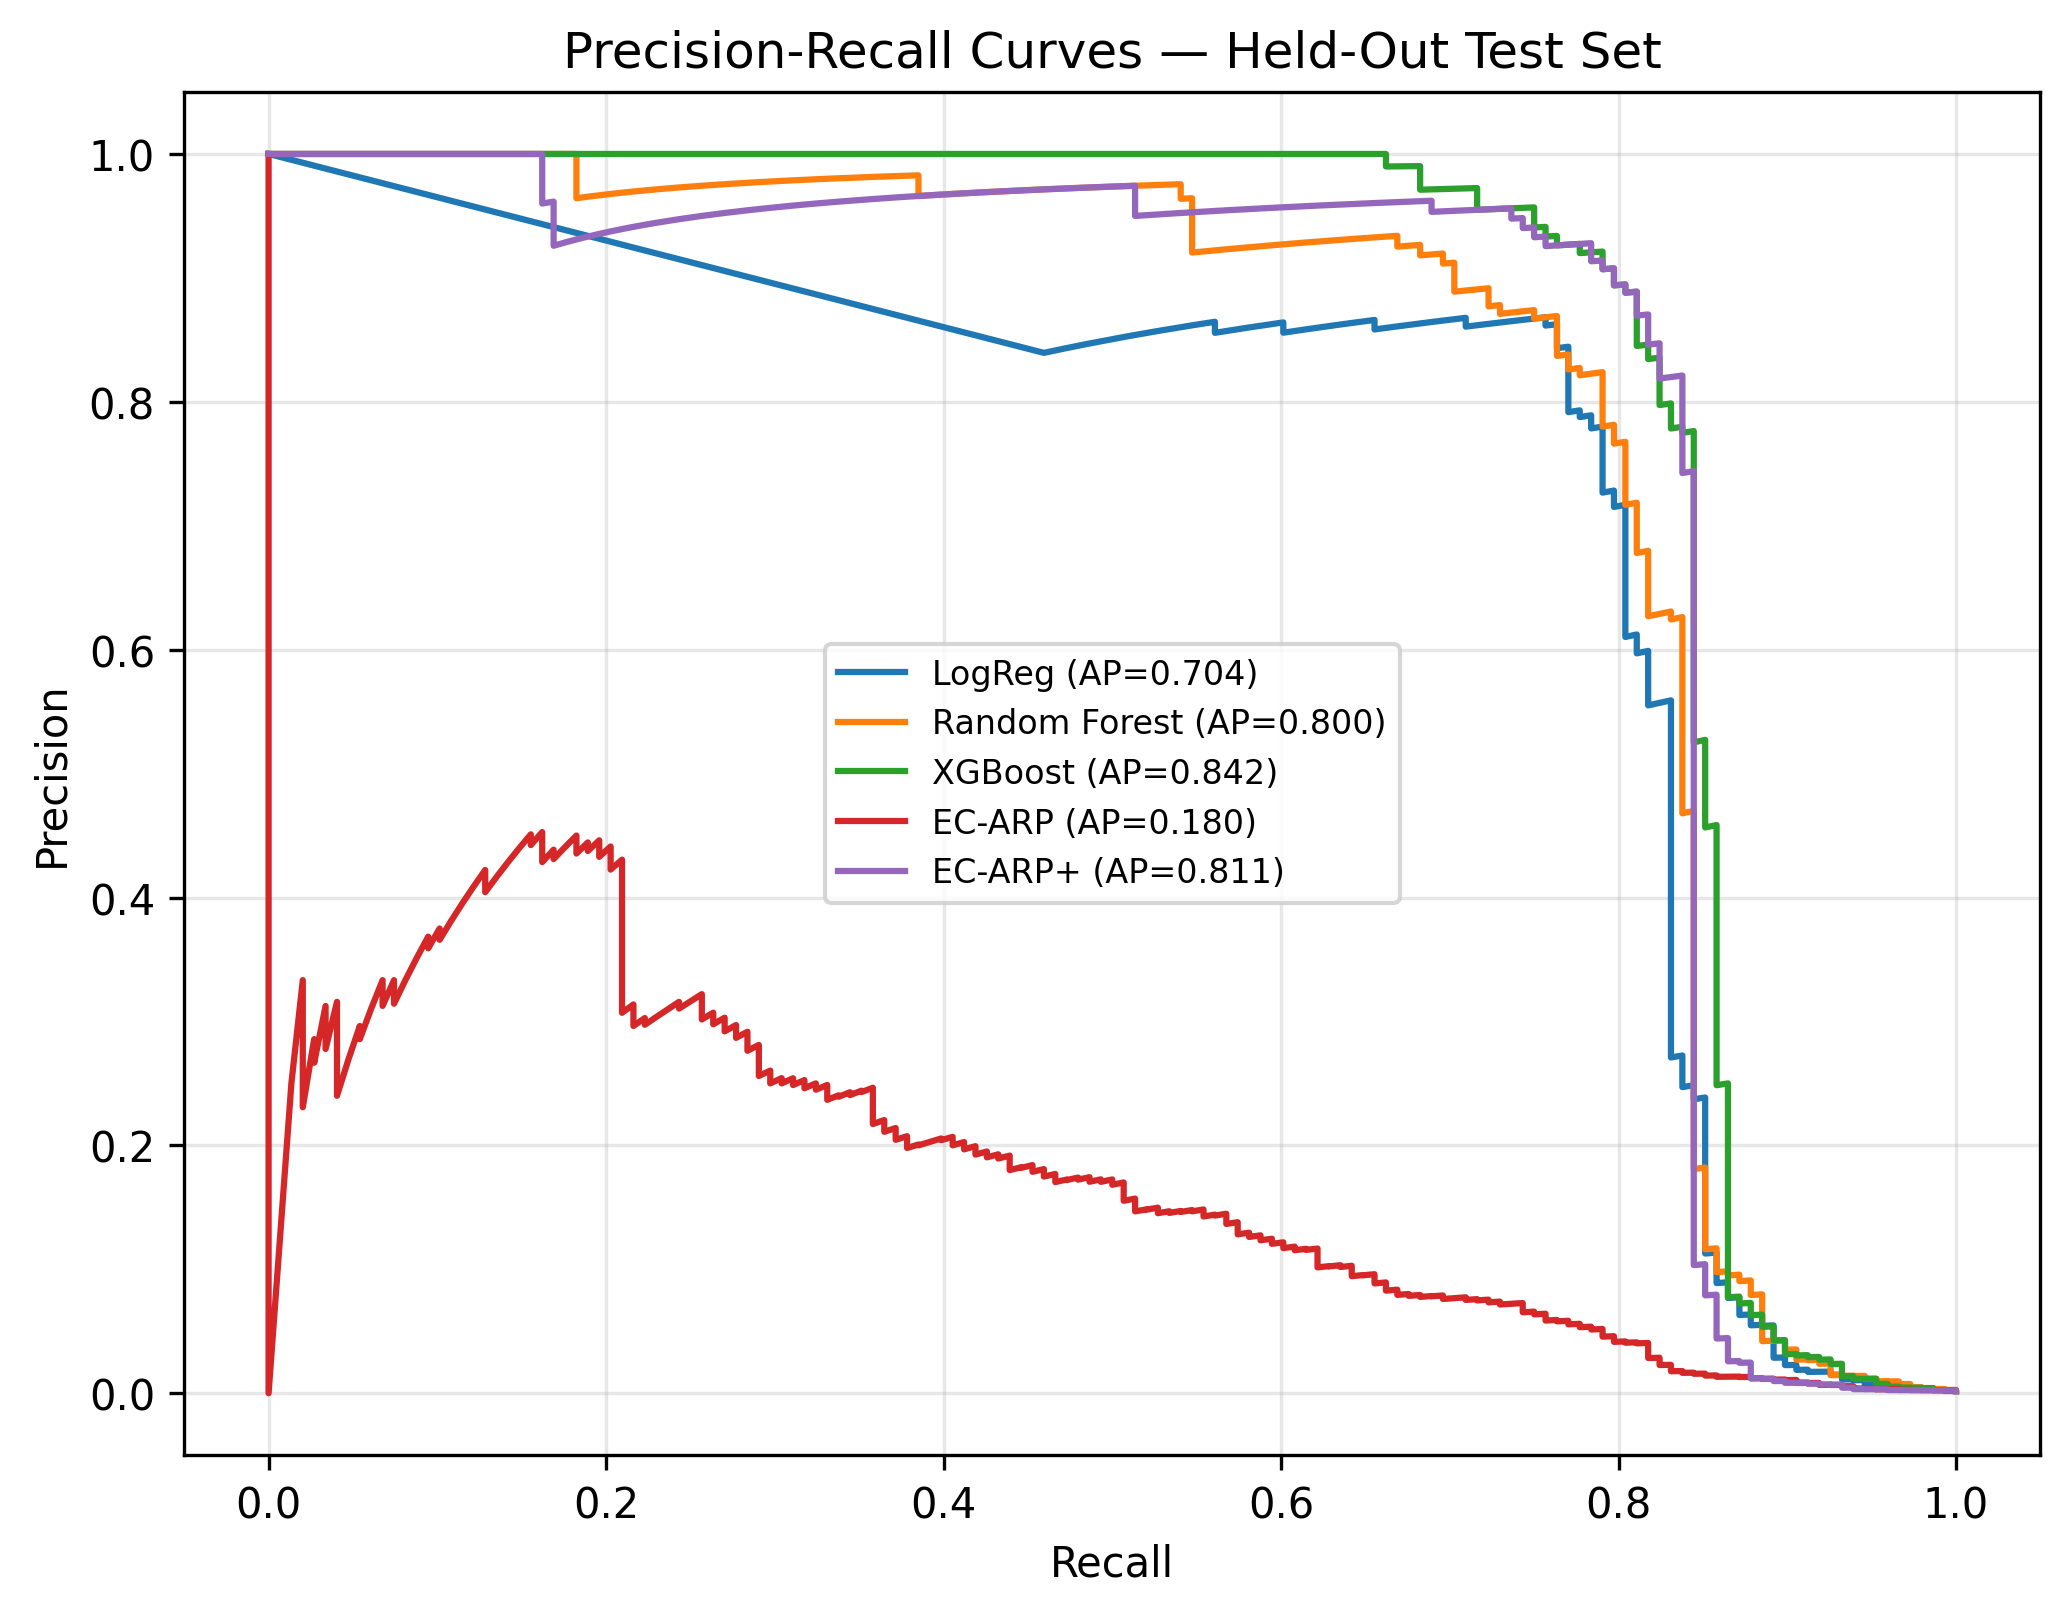
\includegraphics[width=0.95\columnwidth]{figs/model_pr_curves.png}
\caption{Precision--recall curves on the held-out test set. AP values in the legend correspond to the PR-AUC column of Table~\ref{tab:model-comparison}.}
\label{fig:pr-curves}
\end{figure}

\begin{figure}[!t]
\centering
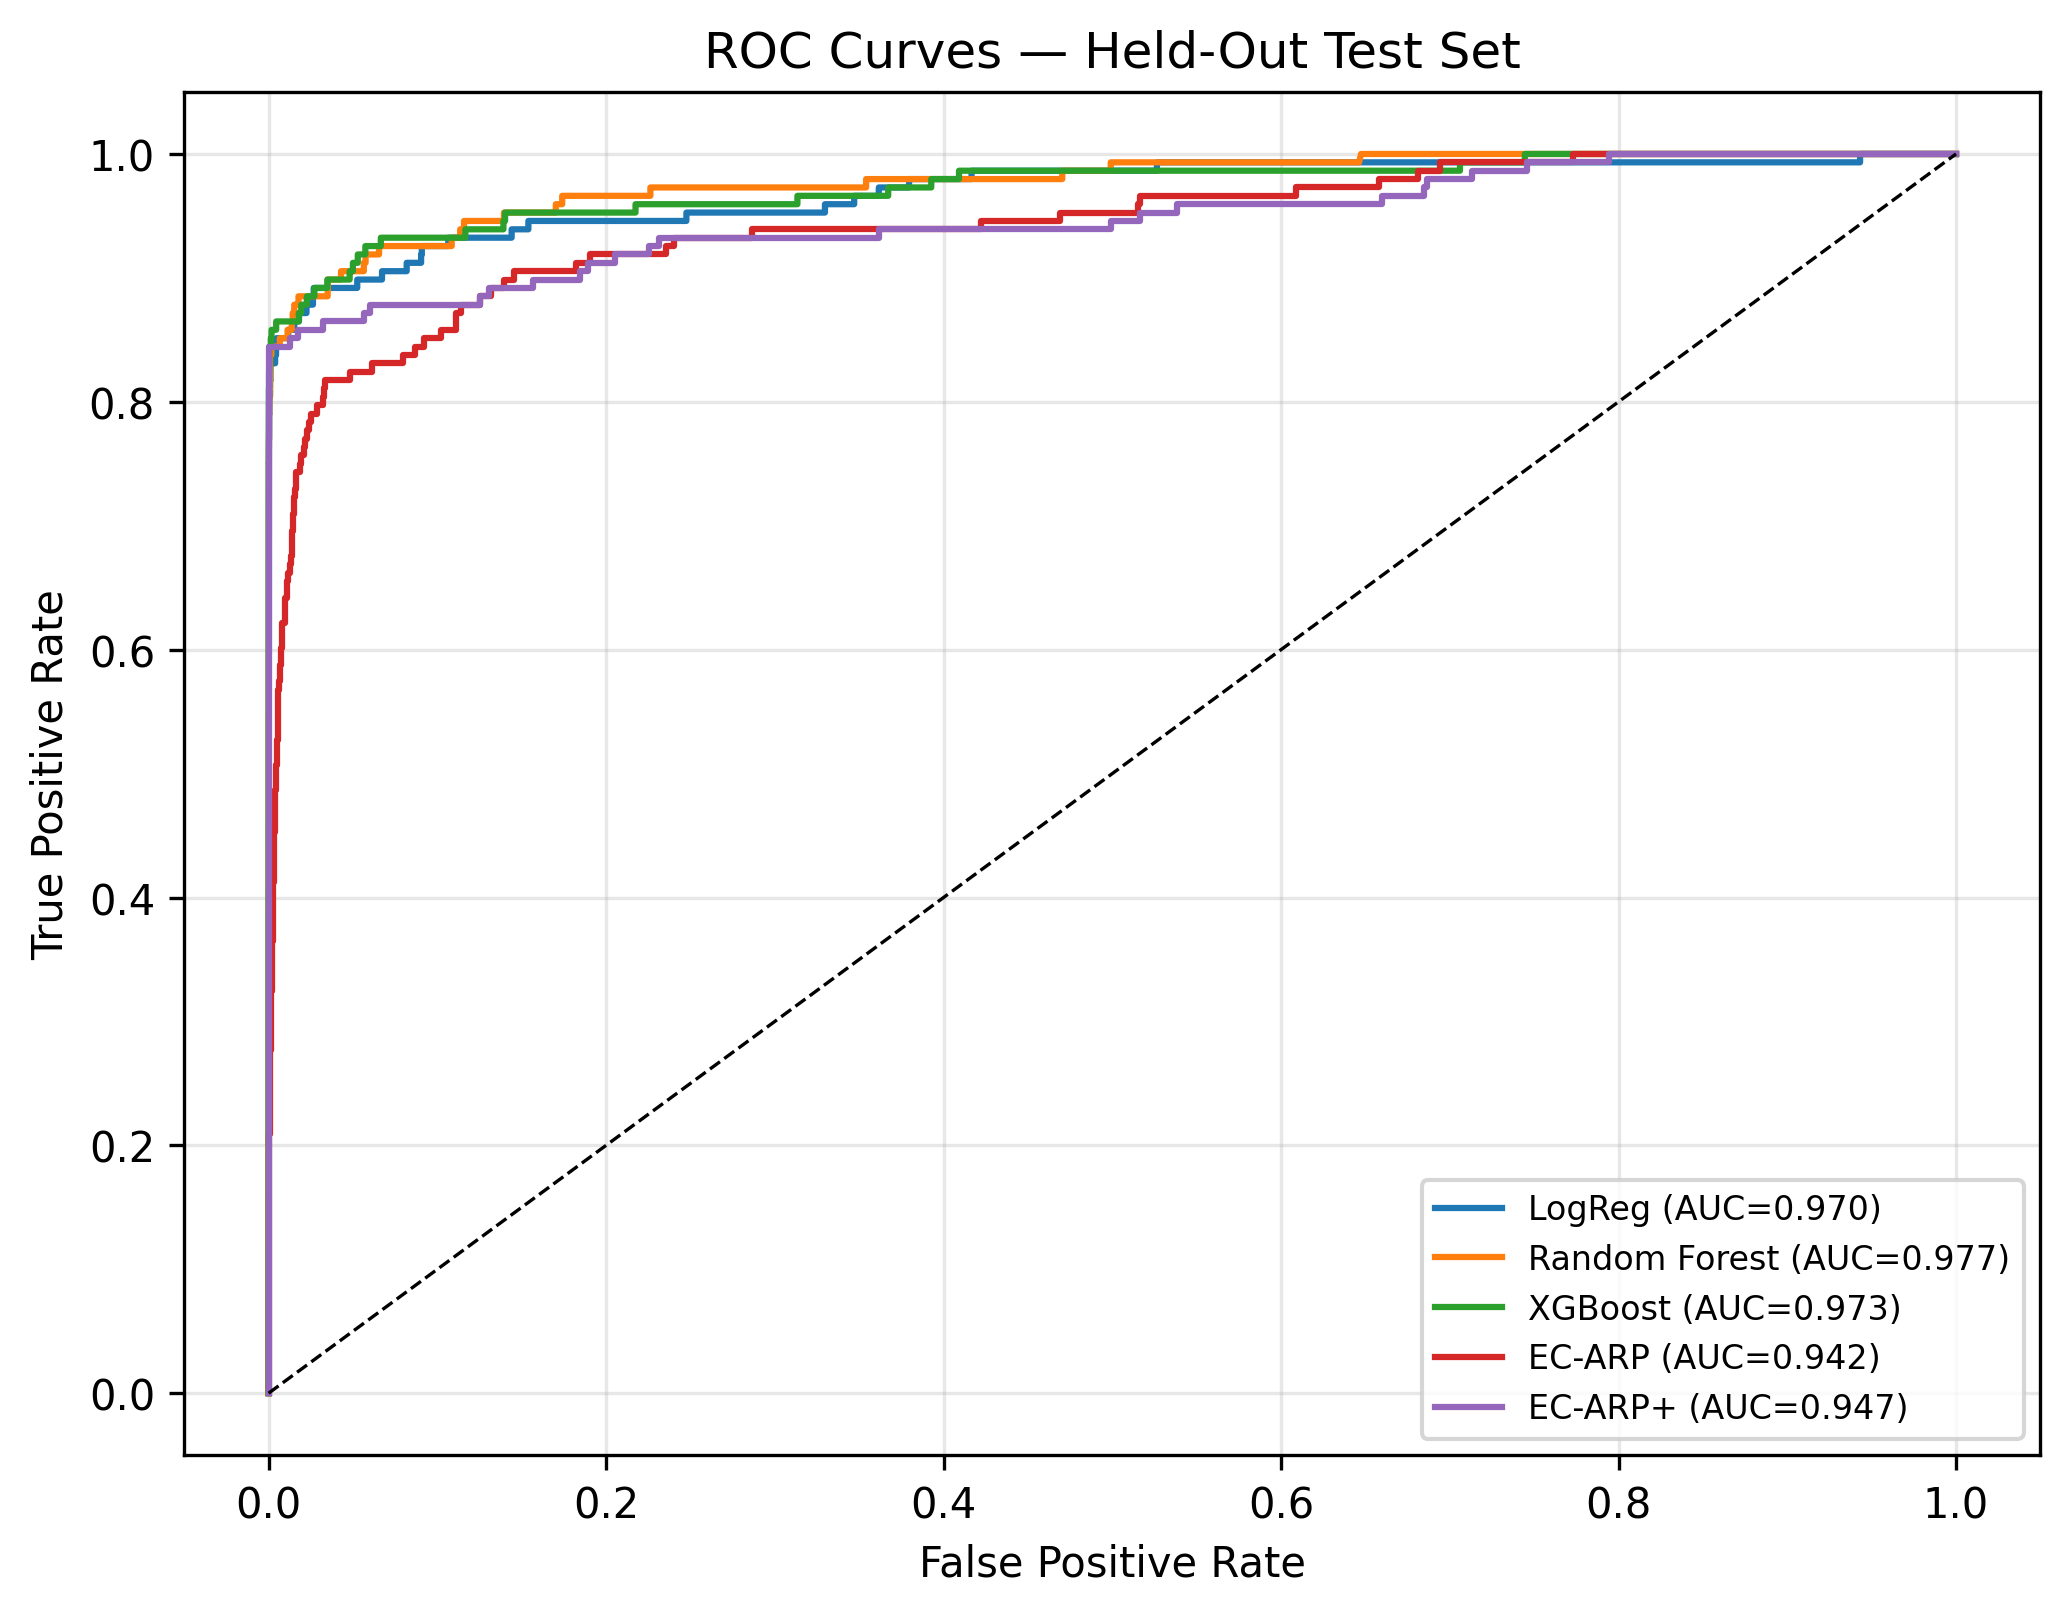
\includegraphics[width=0.95\columnwidth]{figs/model_roc_curves.png}
\caption{ROC curves on the held-out test set.}
\label{fig:roc-curves}
\end{figure}

\subsubsection{Calibrated weights and their interpretation}

Table~\ref{tab:weights} reports the empirically-calibrated weights for both EC-ARP and EC-ARP+, constrained to be non-negative and to sum to one. For EC-ARP, calibration places 68.1\% of the weight on the behavioural-deviation term $b(x_r)$ and 31.9\% on the anomaly term $a(x_r)$; the control-rule term $c(x_r)$ and the frequency/severity term $f(x_r)$ both receive a calibrated weight of zero. For EC-ARP+, the supervised signal dominates ($w_5=0.837$), with the anomaly term retaining modest weight (0.148) and the behavioural and control-rule terms reduced to near zero (0.005 and 0.010 respectively); the frequency/severity term again receives zero weight. Figure~\ref{fig:weights} plots the EC-ARP+ weights.

\begin{table}[!t]
\caption{Empirically Calibrated Weights (non-negative, sum to one)}
\label{tab:weights}
\centering
\scriptsize
\begin{tabular}{l c c}
\toprule
\textbf{Component} & \textbf{EC-ARP} & \textbf{EC-ARP+} \\
\midrule
$w_1$ (anomaly, $a$) & 0.319 & 0.148 \\
$w_2$ (behavioural, $b$) & 0.681 & 0.005 \\
$w_3$ (control rule, $c$) & 0.000 & 0.010 \\
$w_4$ (frequency/severity, $f$) & 0.000 & 0.000 \\
$w_5$ (supervised, out-of-fold XGBoost) & -- & 0.837 \\
\bottomrule
\end{tabular}
\end{table}

\begin{figure}[!t]
\centering
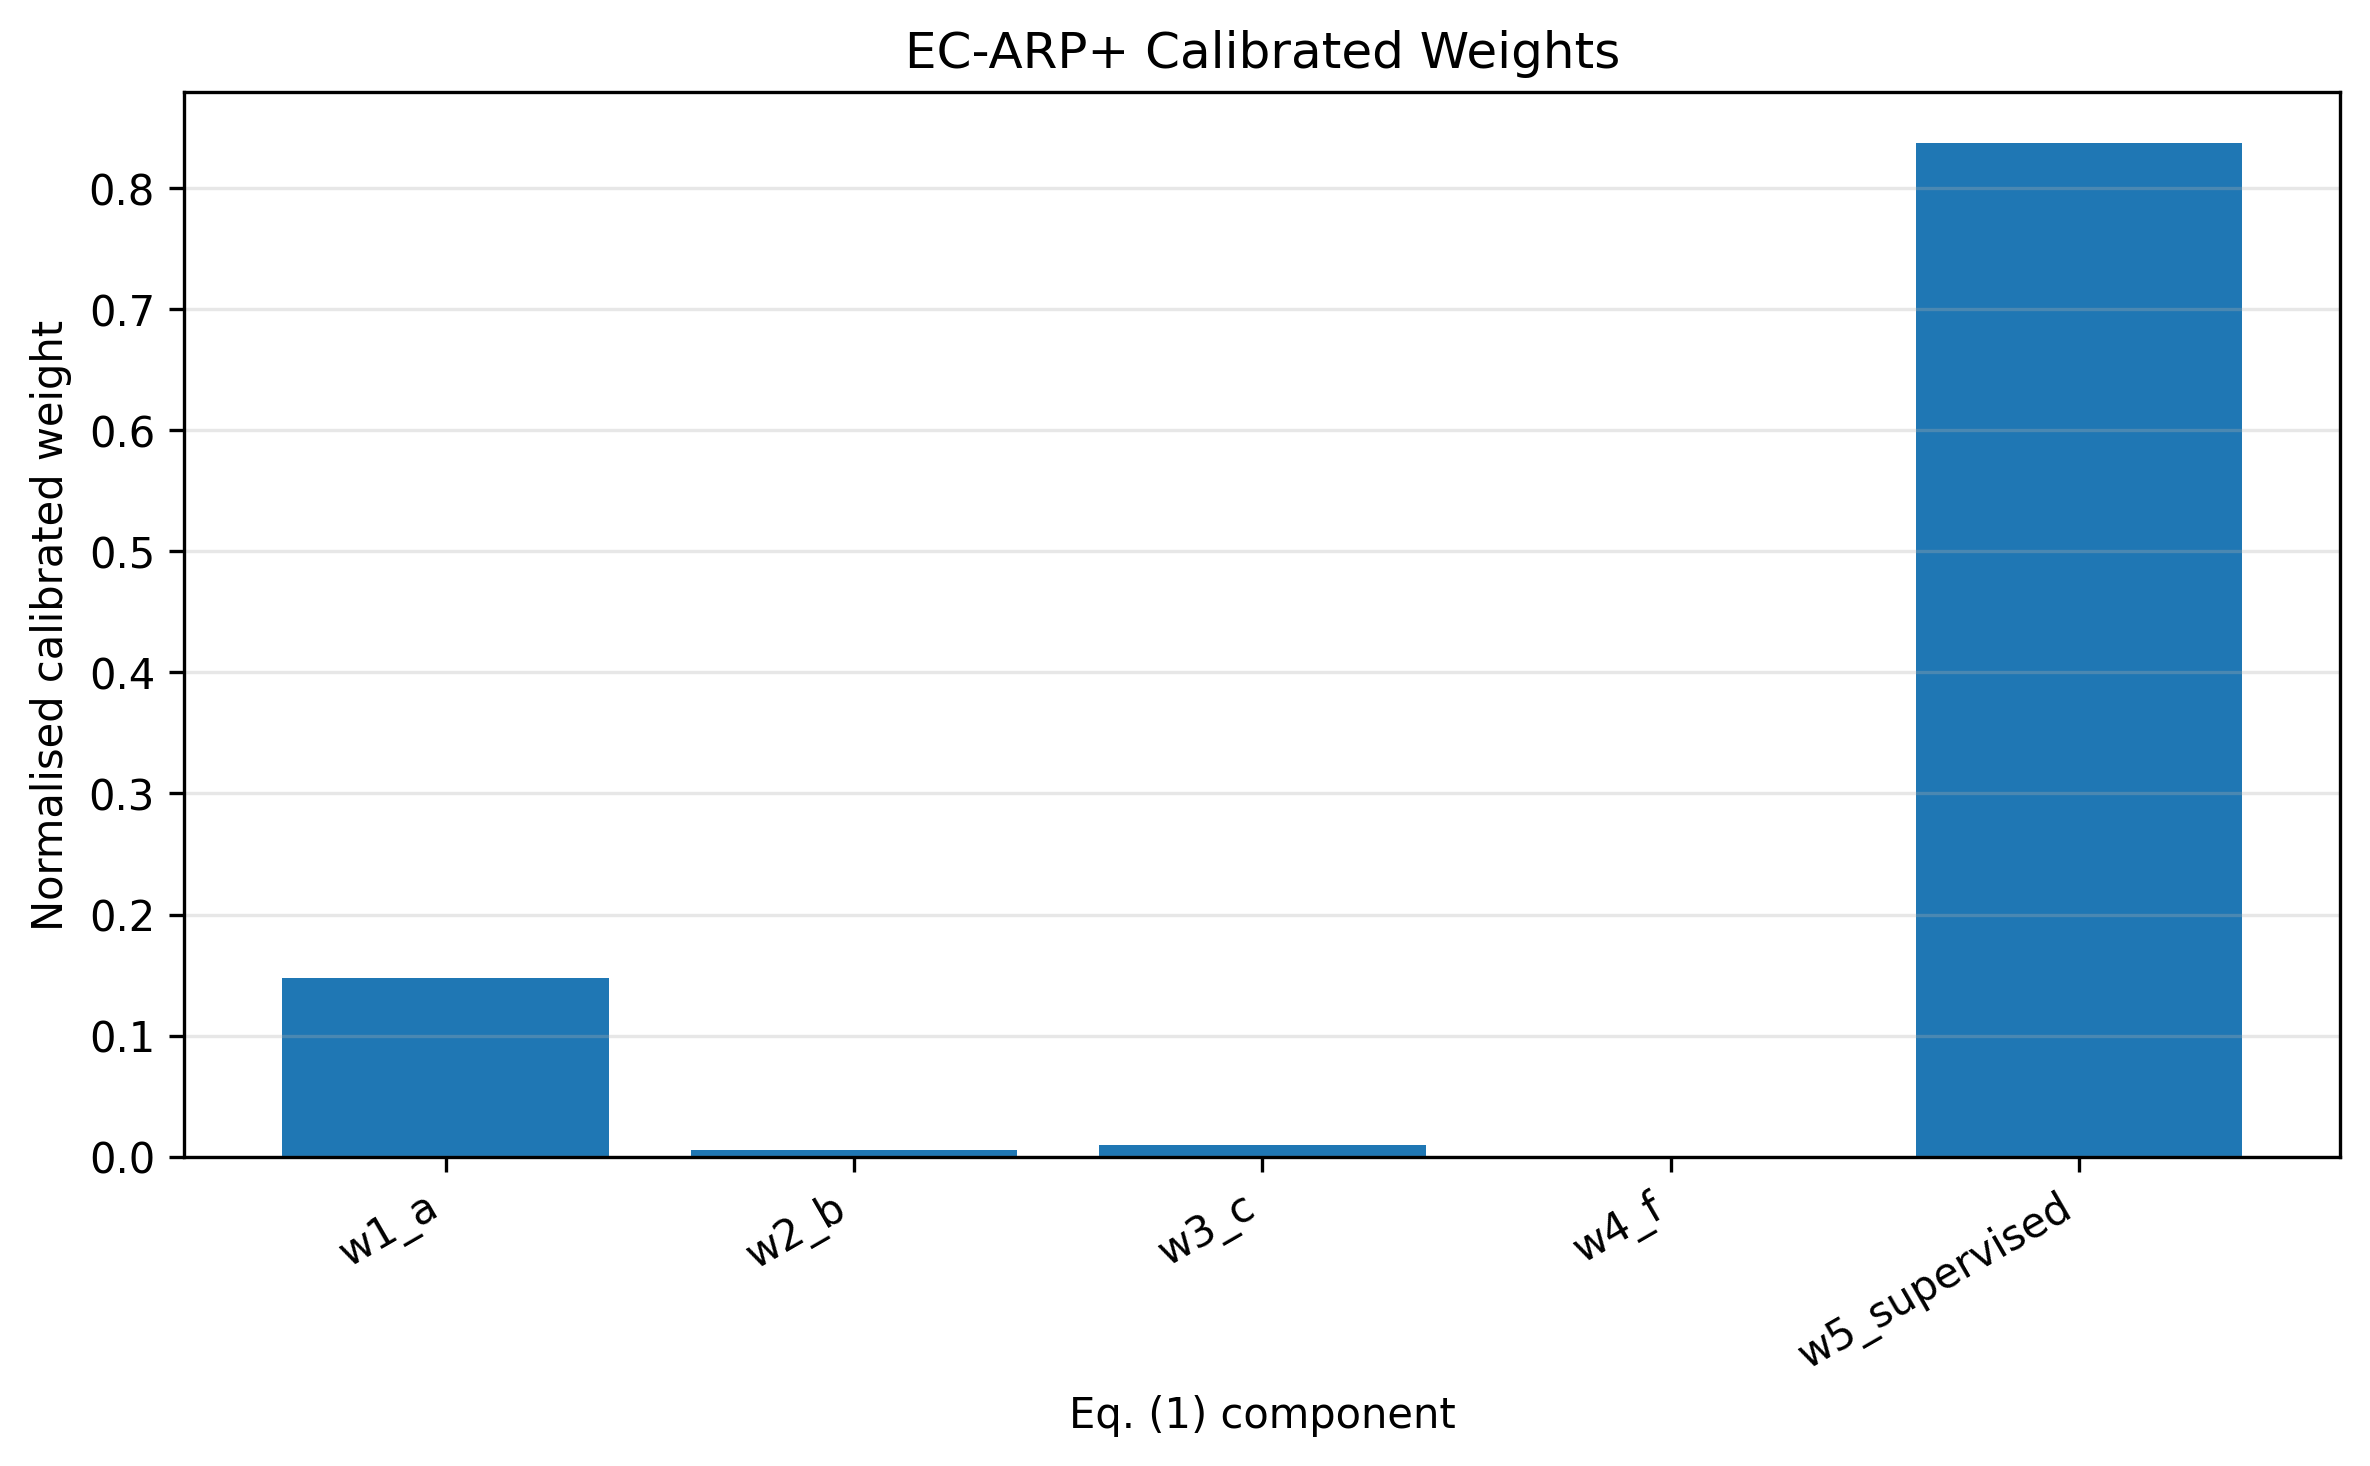
\includegraphics[width=0.95\columnwidth]{figs/model_calibrated_weights.png}
\caption{EC-ARP+ calibrated weights across the five stacked signals.}
\label{fig:weights}
\end{figure}

This pattern must be interpreted carefully. It does \emph{not} show that control-rule or frequency/severity signals are inherently uninformative for fraud detection; rather, it shows that \emph{as operationalised here} -- a simple percentile/off-hours rule for $c(x_r)$ and an amount/local-density composite for $f(x_r)$ -- these two signals carried little additional discriminative power once the anomaly and behavioural (or, for EC-ARP+, the supervised) signals were already included. A more sophisticated instantiation of $c(x_r)$ and $f(x_r)$ -- for example, rules derived from genuine internal-control violations on primary audit data, rather than a percentile/time-window proxy on an anonymised card-transaction benchmark -- might behave differently; this is flagged explicitly as a limitation of the present validation (Section~\ref{sec:limitations}) rather than a general finding about red-flag rule design.

The comparison yields a substantive, honest finding for audit practice: the proposed framework's practical value in this validation comes almost entirely from including a non-linear, supervised signal. A purely unsupervised, rule-based instantiation of Eq.~\eqref{eq:risk} (EC-ARP) is not competitive with standard supervised baselines. EC-ARP+ narrows this gap substantially and, at the top-1\% audit-capacity threshold considered most practically relevant, is close to plain XGBoost -- while remaining decomposable into the four taxonomy-aligned signals plus one supervised term, which is a genuine advantage for auditability and for communicating \emph{why} a transaction was flagged, relative to an undecomposed black-box score. This is an accuracy-versus-decomposability trade-off, not a claim of superiority, and is presented as such.

\section{Ethical Considerations}
\label{sec:ethics}

The reviewed literature raises persistent ethical concerns around algorithmic bias, fairness and transparency in AI-based audit and fraud-detection systems \citep{landers2023,baeyaert2025}, and these concerns extend directly to the empirical validation reported in Section~\ref{sec:empirical-results}. First, class-imbalance correction (class weighting in the baselines; the meta-learner calibration in EC-ARP/EC-ARP+) changes which transactions are flagged, and any deployment on real customer data would need to assess whether flagging rates differ systematically across protected characteristics not present in this anonymised benchmark. Second, the supervised component that drives most of EC-ARP+'s performance is a gradient-boosted ensemble, which is less directly interpretable than the four hand-specified Eq.~\eqref{eq:risk} terms; organisations adopting a stacked architecture of this kind should retain the capacity to explain individual flags (for example via the decomposed EC-ARP terms alongside the supervised score) rather than relying on the composite score alone. Third, because V1--V28 in the validation dataset are anonymised PCA components, this study cannot assess whether the anomaly and behavioural signals correlate with legally or ethically protected attributes; this assessment is essential before any similar architecture is deployed on primary audit or customer data, and is identified explicitly as a precondition for real-world use rather than a solved problem here. Fourth, consistent with the reviewed literature's call for standardised algorithmic-audit protocols \citep{akula2021}, any operational deployment of EC-ARP/EC-ARP+ should be accompanied by documented model cards, a defined recalibration cadence, and human review of escalated cases rather than automated action on the composite score alone.

\section{Conclusion and Policy Recommendations}
\label{sec:conclusion}

\subsection{Conclusion}

This research examined the impact of business analytics on audit and fraud detection across different institutional contexts, and, in its second component, operationalised and empirically tested a composite prioritisation framework rather than leaving it purely conceptual. Five things are established. First, data-driven methods help organisations shift from conventional, retrospective practices towards real-time, predictive and risk-oriented auditing; the analytics-maturity synthesis (Section~\ref{sec:maturity}) shows the reported evolution from fundamental descriptive tools to sophisticated prescriptive systems, alongside reported improvements in anomaly-detection accuracy and fraud-prevention outcomes. Second, the assessment of tool-specific implementations depicts complex trade-offs among usability, detection efficacy, visualisation features and institutional readiness, and the structural analysis of red-flag indicators reinforces the value of classifying fraud symptoms by data complexity and contextual traceability. Third, sectoral analysis indicates significant disparities in adoption, shaped by regulatory pressure, technological proficiency and organisational priorities; comparative frameworks show that analytics-driven audits offer expanded scope, immediate reactivity and improved risk traceability relative to conventional sampling-based auditing. Fourth, the proposed AI-assisted red-flag prioritisation framework (Section~\ref{sec:framework}) has now been operationalised and empirically tested on a public 284,807-transaction benchmark: a stacked hybrid instantiation (EC-ARP+) is competitive with, though it does not exceed, a plain gradient-boosted baseline, while the purely unsupervised instantiation (EC-ARP) under-performs, with its calibrated weights collapsing the control-rule and frequency/severity terms to zero on this dataset. Fifth, enduring issues persist across both components of this study: infrastructure fragmentation, expertise deficiencies among audit professionals, and ethical concerns about algorithmic bias and transparency (Section~\ref{sec:ethics}).

This research enhances audit theory by showing how business analytics may convert conventional audits into real-time, risk-oriented systems, and by demonstrating -- through an actual empirical test -- what is and is not achieved when a conceptual prioritisation framework is operationalised on real transaction data. It contributes to the literature by systematically compiling and comparing audit tools, categorising red-flag indicators, examining sector-specific adoption patterns, and providing a framework that connects analytics, governance and fraud detection to an empirically testable architecture. These contributions are intended to help scholars and practitioners understand the practical application of audit analytics and to facilitate further inquiry into intelligent auditing, including replication of the validation protocol on primary audit data.

\subsection{Policy Recommendations}

Policymakers, regulators and organisational leaders should consider the following initiatives to act on the findings of this analytics-enhanced audit research. Standardisation of algorithmic audit protocols is essential: regulatory authorities should formulate internationally accepted standards for artificial intelligence and machine learning in auditing, prioritising transparent audit processes to ensure adherence to ethical and legal requirements. Investment in digital audit infrastructure is necessary, including upgrading legacy systems and adopting cloud-based audit platforms, real-time data streams and centralised data governance. Development of competence and interdisciplinary training should be reinforced through a new auditor-competency framework addressing SQL, Python, inferential statistics and data visualisation, supported by government and professional-body funding for certificates, workshops and university-level programmes. Fraud-simulation environments -- ``fraud sandboxes'' -- can provide secure, regulated settings in which to evaluate the effectiveness and equity of fraud-detection algorithms such as EC-ARP/EC-ARP+, improving innovation and regulatory scrutiny while reducing unexpected legal exposure for institutions. Implementation frameworks specific to sectors are also required: public-sector entities, non-profit organisations and small to medium-sized enterprises need streamlined, modular and scalable frameworks suited to constrained resources and staffing. Finally, organisations should integrate analytical outputs into formal governance structures, with systematic feedback mechanisms across audit teams, IT departments and executive leadership, so that identified anomalies inform upstream policy decisions and model precision improves through organisational learning.

\subsection{Limitations and Future Research}
\label{sec:limitations}

The findings are qualified by several limitations, separated into those concerning the review component and those concerning the empirical validation component.

\emph{Review limitations.} This is an integrative review of secondary sources for RQ1--RQ4 and contributes no primary empirical audit data for those questions; its conclusions reflect the state of the reviewed literature rather than independently measured outcomes, and no causal effects can be established from it. The evidence base is heterogeneous, combining peer-reviewed research with industry and professional reports of varying rigour. The review is subject to publication and selection bias, and coverage is weighted towards English-language sources, which may under-represent practice in other regions and languages. The database set, while broad, is not exhaustive and excludes some specialist venues. During reference verification, one in-text citation (Wolniak, 2024, cited for the finding that data-quality deficiencies are the primary reported obstacle to analytics adoption) could not be matched to a complete bibliographic entry and is flagged in the reference list as requiring author confirmation rather than presented with fabricated details.

\emph{Empirical validation limitations.} The validation in Section~\ref{sec:empirical-method} uses a single public benchmark dataset of anonymised card transactions, not primary audit, general-ledger, procurement or financial-statement data; external validity to internal-audit contexts specifically requires testing on such data. The dataset contains no customer or entity identifiers, so the behavioural-deviation ($b$) and frequency ($f$) signals are computed as dataset-level unsupervised proxies rather than true per-account longitudinal profiles. Twenty-eight of the 30 predictor features are already anonymised principal components, limiting the business interpretability of the anomaly and rule signals and precluding testing of the taxonomy's structural-anomaly, documentation-discrepancy and relational-fraud clusters, none of which are represented in this dataset. The control rule $c(x_r)$ was defined as a simple, reproducible percentile/off-hours proxy for illustrative and methodological purposes, not as a validated internal-control rule. Results come from a single stratified 70/30 train/test split with a fixed random seed rather than repeated cross-validation with confidence intervals. Credit-card transaction fraud is structurally different from the financial-statement and procurement fraud that much of the reviewed literature addresses, so the empirical results should be read as a methodological proof of concept for the validation protocol, not as a direct performance claim for financial-statement audit.

These limitations define a research agenda. Future work should (i) replicate the validation protocol on primary audit-log, procurement or general-ledger data with genuine entity identifiers and internal-control rules, ideally within a fraud-sandbox arrangement that permits controlled access to sensitive data; (ii) report repeated cross-validated confidence intervals rather than a single split; (iii) test the framework's explainability and fairness properties, particularly given the bias concerns noted in Section~\ref{sec:ethics}; (iv) extend the taxonomy-to-feature mapping to the structural-anomaly, documentation-discrepancy and relational-fraud clusters using data sources that actually contain such signals (e.g., ledger reconciliation data, document metadata, or relationship graphs); and (v) investigate the organisational conditions -- skills, data governance and change management -- that this study identifies as decisive but does not evaluate jointly with model performance.

\section*{Code and Data Availability}
All feature-engineering and model-training code used to produce Table~\ref{tab:model-comparison}, Table~\ref{tab:weights} and Figures~\ref{fig:pr-curves}--\ref{fig:weights} is released alongside this manuscript as two Python scripts: a dataset-analysis script and a model-training script implementing EC-ARP, EC-ARP+ and all four baselines, together with the raw output files (CSV/JSON metrics and PNG figures) from two independent runs (local and Kaggle) that produced numerically consistent results. The dataset is the publicly available ULB ``Credit Card Fraud Detection'' benchmark \citep{dalpozzolo2015}. Random seeds are fixed (\texttt{random\_state}=42) for reproducibility; exact figures will shift marginally under a different seed or resampling.

\noindent Bibliographic details were checked against public sources where possible. The entry marked \rvr\ could not be located and requires author confirmation before submission.

\begin{thebibliography}{00}

\bibitem[Abdelwahed et al.(2024)]{abdelwahed2024} Abdelwahed, A.\ S., Abu-Musa, A.\ A., Moubarak, H., \& Badawy, H.\ A.\ (2024). The use of big data and analytics in external auditing: Does audit firm size matter? Evidence from a developing country. \emph{South African Journal of Accounting Research}, 38(2), 113--145.

\bibitem[Adejumo and Ogburie(2025)]{adejumo2025} Adejumo, A., \& Ogburie, C.\ (2025). Financial statement manipulation: Ethical and regulatory perspectives. \emph{GSC Advanced Research and Reviews}, 22(3), 252--264.

\bibitem[Adepoju et al.(2022)]{adepoju2022} Adepoju, A.\ H., Austin-Gabriel, B., Hamza, O., \& Collins, A.\ (2022). Advancing monitoring and alert systems: A proactive approach to improving reliability in complex data ecosystems. \emph{IRE Journals}, 5(11), 281--282.

\bibitem[Aivaz et al.(2024)]{aivaz2024} Aivaz, K.\ A., Florea, I.\ O., \& Munteanu, I.\ (2024). Economic fraud and associated risks: An integrated bibliometric analysis approach. \emph{Risks}, 12(5), 74.

\bibitem[Akter(2025)]{akter2025} Akter, M.\ (2025). \emph{Enhancing SME Competitiveness: The Role of Business Intelligence in Data-Driven Decision-Making} (Bachelor's thesis).

\bibitem[Akula and Garibay(2021)]{akula2021} Akula, R., \& Garibay, I.\ (2021). Audit and assurance of AI algorithms: A framework to ensure ethical algorithmic practices in artificial intelligence. \emph{arXiv preprint arXiv:2107.14046}.

\bibitem[Alex-Omiogbemi et al.(2024)]{alexomiogbemi2024} Alex-Omiogbemi, A.\ A., Sule, A.\ K., Omowole, B.\ M., \& Owoade, S.\ J.\ (2024). Conceptual framework for advancing regulatory compliance and risk management in emerging markets through digital innovation. \emph{World Journal of Advanced Research and Reviews}, 24(3), 1155--1162.

\bibitem[Ayodeji(2024)]{ayodeji2024} Ayodeji, I.\ A.\ (2024). \emph{Fraud Detection and Prevention in the Nigerian Financial Industry} (Doctoral dissertation, Walden University).

\bibitem[Baeyaert(2025)]{baeyaert2025} Baeyaert, J.\ (2025). Harmonizing creativity and ethics in AI systems. \emph{AI and Ethics}, 1--21.

\bibitem[Balogun et al.(2021)]{balogun2021} Balogun, E.\ D., Ogunsola, K.\ O., \& Samuel, A.\ (2021). A risk intelligence framework for detecting and preventing financial fraud in digital marketplaces. \emph{Iconic Research and Engineering Journals}, 4(8), 134--149.

\bibitem[Bello et al.(2024)]{bello2024} Bello, H.\ O., Ige, A.\ B., \& Ameyaw, M.\ N.\ (2024). Adaptive machine learning models: Concepts for real-time financial fraud prevention in dynamic environments. \emph{World Journal of Advanced Engineering Technology and Sciences}, 12(2), 021--034.

\bibitem[Breiman(2001)]{breiman2001} Breiman, L.\ (2001). Random forests. \emph{Machine Learning}, 45(1), 5--32.

\bibitem[Carre\~no(2024)]{carreno2024} Carre\~no, A.\ M.\ (2024). \emph{Strategic Alignment in Program Management: A Framework for Sustainable Business Transformation}. Institute for Change Leadership and Business Transformation.

\bibitem[Chen and Guestrin(2016)]{chen2016} Chen, T., \& Guestrin, C.\ (2016). XGBoost: A scalable tree boosting system. In \emph{Proceedings of the 22nd ACM SIGKDD International Conference on Knowledge Discovery and Data Mining} (pp. 785--794).

\bibitem[Chowdhury and Masum(2025)]{chowdhury2025} Chowdhury, R.\ H., \& Masum, A.\ A.\ (2025). Utilizing business analytics to combat financial fraud and enhance economic integrity. \emph{International Journal of Science and Research Archive}, 14(1), 134--145.

\bibitem[Dal Pozzolo et al.(2015)]{dalpozzolo2015} Dal Pozzolo, A., Caelen, O., Johnson, R.\ A., \& Bontempi, G.\ (2015). Calibrating probability with undersampling for unbalanced classification. In \emph{2015 IEEE Symposium Series on Computational Intelligence} (pp. 159--166).

\bibitem[Darwin(2024)]{darwin2024} Darwin, K.\ (2024). Strengthening public and private accountability through digital forensic accounting. \emph{Sinergi International Journal of Accounting and Taxation}, 2(4), 225--238.

\bibitem[Darwish(2024)]{darwish2024} Darwish, D.\ (Ed.). (2024). \emph{Emerging Trends in Cloud Computing Analytics, Scalability, and Service Models}. IGI Global.

\bibitem[Douglas(2024)]{douglas2024} Douglas, F.\ (2024). \emph{Can Small Businesses Deter Fraud? A Qualitative Examination of Preventive and Detective Internal Control Strategies} (Doctoral dissertation, National University).

\bibitem[Ebirim et al.(2024)]{ebirim2024} Ebirim, G.\ U., Unigwe, I.\ F., Oshioste, E.\ E., Ndubuisi, N.\ L., Odonkor, B., \& Asuzu, O.\ F.\ (2024). Innovations in accounting and auditing: A comprehensive review of current trends and their impact on US businesses. \emph{International Journal of Science and Research}, 11, 965--974.

\bibitem[ElDahshan et al.(2024)]{eldahshan2024} ElDahshan, K.\ A., Abutaleb, G.\ E., Elemary, B.\ R., Ebeid, E.\ A., \& AlHabshy, A.\ A.\ (2024). An optimized intelligent open-source MLaaS framework for user-friendly clustering and anomaly detection. \emph{The Journal of Supercomputing}, 80(18), 26658--26684.

\bibitem[Elumilade et al.(2024)]{elumilade2024} Elumilade, O.\ O., Ogundeji, I.\ A., Ozoemenam, G., Omokhoa, H.\ E., \& Omowole, B.\ M.\ (2024). Advancing audit efficiency through statistical sampling and compliance best practices in financial reporting. \emph{IRE Journals}, 7(9), 434--437.

\bibitem[Faccia and Petratos(2024)]{faccia2024} Faccia, A., \& Petratos, P.\ (2024). Big data applications in accounting information systems. In \emph{Proceedings of the 2024 9th International Conference on Big Data and Computing} (pp. 1--7).

\bibitem[Fernandes et al.(2019)]{fernandes2019} Fernandes Jr., G., Rodrigues, J.\ J., Carvalho, L.\ F., Al-Muhtadi, J.\ F., \& Proen\c{c}a Jr., M.\ L.\ (2019). A comprehensive survey on network anomaly detection. \emph{Telecommunication Systems}, 70(3), 447--489.

\bibitem[Fiolleau et al.(2024)]{fiolleau2024} Fiolleau, K., MacTavish, C., Osecki, E., \& Thorne, L.\ (2024). An exploration of technological innovations in the audit industry: Disruption theory applied to a regulated industry. \emph{Accounting Perspectives}, 23(3), 403--445.

\bibitem[George(2022)]{george2022} George, J.\ (2022). Optimizing hybrid and multi-cloud architectures for real-time data streaming and analytics: Strategies for scalability and integration. \emph{World Journal of Advanced Engineering Technology and Sciences}, 7(1), 174--185.

\bibitem[Hamdam et al.(2022)]{hamdam2022} Hamdam, A., Jusoh, R., Yahya, Y., Abdul Jalil, A., \& Zainal Abidin, N.\ H.\ (2022). Auditor judgment and decision-making in big data environment: A proposed research framework. \emph{Accounting Research Journal}, 35(1), 55--70.

\bibitem[Hassan et al.(2023)]{hassan2023} Hassan, A., Salleh, N., Ismail, M.\ N., Ahmad, M.\ N., \& Hussin, A.\ R.\ C.\ (2023). Empirical evaluation of continuous auditing system use: A systematic review. \emph{International Journal of Electrical and Computer Engineering}, 13(1), 796.

\bibitem[Henriques(2024)]{henriques2024} Henriques, J.\ P.\ M.\ (2024). \emph{Audit Compliance and Forensics Frameworks for Improved Critical Infrastructure Protection} (Doctoral dissertation, Universidade de Coimbra).

\bibitem[Hezam et al.(2023)]{hezam2023} Hezam, Y.\ A., Anthonysamy, L., \& Suppiah, S.\ D.\ K.\ (2023). Big data analytics and auditing: A review and synthesis of literature. \emph{Emerging Science Journal}, 7(2), 629--642.

\bibitem[Hilal et al.(2022)]{hilal2022} Hilal, W., Gadsden, S.\ A., \& Yawney, J.\ (2022). Financial fraud: A review of anomaly detection techniques and recent advances. \emph{Expert Systems with Applications}, 193, 116429.

\bibitem[Ilori et al.(2024)]{ilori2024} Ilori, O., Nwosu, N.\ T., \& Naiho, H.\ N.\ N.\ (2024). Advanced data analytics in internal audits: A conceptual framework for comprehensive risk assessment and fraud detection. \emph{Finance \& Accounting Research Journal}, 6(6), 931--952.

\bibitem[Javaid(2024)]{javaid2024} Javaid, H.\ A.\ (2024). Improving fraud detection and risk assessment in financial service using predictive analytics and data mining. \emph{Integrated Journal of Science and Technology}, 1(8).

\bibitem[Johnson-Rokosu and Enobi(2025)]{johnsonrokosu2025} Johnson-Rokosu, S.\ F., \& Enobi, A.\ (2025). Behavioral analytics and forensic accounting: Understanding the human element in fraud. \emph{Journal of Accounting and Financial Management}, 11(5), 93--117.

\bibitem[Joshi and Patel(2021)]{joshi2021} Joshi, A.\ P., \& Patel, B.\ V.\ (2021). Data preprocessing: The techniques for preparing clean and quality data for data analytics process. \emph{Oriental Journal of Computer Science and Technology}, 13(0203), 78--81.

\bibitem[Kothandapani(2025)]{kothandapani2025} Kothandapani, H.\ P.\ (2025). AI-driven regulatory compliance: Transforming financial oversight through large language models and automation. \emph{Emerging Science Research}, 12--24.

\bibitem[Landers and Behrend(2023)]{landers2023} Landers, R.\ N., \& Behrend, T.\ S.\ (2023). Auditing the AI auditors: A framework for evaluating fairness and bias in high stakes AI predictive models. \emph{American Psychologist}, 78(1), 36.

\bibitem[Liu et al.(2008)]{liu2008} Liu, F.\ T., Ting, K.\ M., \& Zhou, Z.-H.\ (2008). Isolation forest. In \emph{2008 Eighth IEEE International Conference on Data Mining} (pp. 413--422).

\bibitem[Lokanan(2024)]{lokanan2024} Lokanan, M.\ (2024). \emph{Harnessing Exploratory Data Analysis for Robust Financial Fraud Detection and Model Enhancement}. Research Square (preprint).

\bibitem[Machireddy(2022)]{machireddy2022} Machireddy, J.\ R.\ (2022). Integrating predictive modeling with policy interventions to address fraud, waste, and abuse (FWA) in US healthcare systems. \emph{Advances in Computational Systems, Algorithms, and Emerging Technologies}, 7(1), 35--65.

\bibitem[Mai(2022)]{mai2022} Mai, L.\ P.\ (2022). \emph{Changes in Competencies, Capabilities, and Decision-Making in the Accounting Profession as a Result of Information Digitalization and Big Data Analytics/Artificial Intelligence} (Master's thesis, Ca' Foscari University of Venice).

\bibitem[Malempati(2025)]{malempati2025} Malempati, M.\ (2025). \emph{The Intelligent Ledger: Harnessing Artificial Intelligence, Big Data, and Cloud Power to Revolutionize Finance, Credit, and Security}. Deep Science Publishing.

\bibitem[Naoufal(2024)]{naoufal2024} Naoufal, G.\ (2024). Continuous auditing/continuous monitoring. In \emph{Continuous Auditing with AI in the Public Sector} (pp. 143--162). CRC Press.

\bibitem[Nogueira et al.(2025)]{nogueira2025} Nogueira, D.\ M., Sim\~oes, M., Ferreira, C., Ribeiro, R.\ P., Mart\'inez-Rego, D., Cai, A., \& Gama, J.\ (2025). Survey on detection of fraudulent documents. \emph{Authorea Preprints}.

\bibitem[Nouri(2024)]{nouri2024} Nouri, Z.\ (2024). \emph{Financial Audit Using Data Analytics} (Master's thesis, Universidade NOVA de Lisboa).

\bibitem[Oko-Odion and Udoh(2024)]{okoodion2024} Oko-Odion, C., \& Udoh, O.\ R.\ (2024). Leveraging technology in internal audit processes for streamlined management and risk oversight. \emph{International Journal of Science and Research Archive}, 13(2), 3077--3100.

\bibitem[Oliveira and Ribeiro(2022)]{oliveira2022} Oliveira, J., \& Ribeiro, P.\ J.\ (2022). Technological developments and new hybrid roles in accounting and finance. In \emph{The Routledge Handbook of Accounting Information Systems} (pp. 156--170). Routledge.

\bibitem[Pamisetty(2021)]{pamisetty2021} Pamisetty, V.\ (2021). Integrating predictive analytics and IT infrastructure for advanced government financial management and fraud detection. \emph{SSRN Working Paper}.

\bibitem[Panchapakesan et al.(2025)]{panchapakesan2025} Panchapakesan, A., Anandaram, H., Sridevi, L., Sathish, K.\ M., Dhivya, P., Parameswari, S., \& Kapadia, H.\ (2025). Enhancing audit effectiveness through strategic data analytics. In \emph{Machine Learning and Modeling Techniques in Financial Data Science} (pp. 231--252). IGI Global.

\bibitem[Pinto(2024)]{pinto2024} Pinto, A.\ R.\ O.\ (2024). \emph{A Framework for Leveraging IT Audit Using Artificial Intelligence} (Master's thesis, Universidade NOVA de Lisboa).

\bibitem[Pizzini and Sterin(2025)]{pizzini2025} Pizzini, M., \& Sterin, M.\ (2025). The relation between cash reserves, governance, and donations in nonprofit organizations. \emph{Journal of Accounting, Auditing \& Finance}, 40(1), 139--164.

\bibitem[Popoola(2023)]{popoola2023} Popoola, N.\ T.\ (2023). Big data-driven financial fraud detection and anomaly detection systems for regulatory compliance and market stability. \emph{International Journal of Computer Applications Technology and Research}, 12(9), 32--46.

\bibitem[Prosper(2025)]{prosper2025} Prosper, J.\ (2025). \emph{Data Conversion Failures and Their Influence on Fraud Detection and Audit Accuracy in Medicare and Medicaid} (preprint).

\bibitem[Qatawneh(2024)]{qatawneh2024} Qatawneh, A.\ M.\ (2024). The role of artificial intelligence in auditing and fraud detection in accounting information systems: Moderating role of natural language processing. \emph{International Journal of Organizational Analysis}.

\bibitem[Rumasukun(2024)]{rumasukun2024} Rumasukun, M.\ R.\ (2024). Developing auditor competencies through continuous training and education. \emph{Golden Ratio of Auditing Research}, 4(1), 14--23.

\bibitem[Sarkola(2023)]{sarkola2023} Sarkola, M.\ (2023). \emph{Developing Global System-Based Indirect Purchasing in the Case Company} (Master's thesis, LUT University).

\bibitem[Sewpersadh(2025)]{sewpersadh2025} Sewpersadh, N.\ S.\ (2025). Adaptive structural audit processes as shaped by emerging technologies. \emph{International Journal of Accounting Information Systems}, 56, 100735.

\bibitem[Solano and Cruz(2024)]{solano2024} Solano, M.\ C., \& Cruz, J.\ C.\ (2024). Integrating analytics in enterprise systems: A systematic literature review of impacts and innovations. \emph{Administrative Sciences}, 14(7), 138.

\bibitem[Sutisna(2025)]{sutisna2025} Sutisna, E.\ (2025). Evaluating security risks and the impact of analytic technology on the audit process. \emph{Advances in Managerial Auditing Research}, 3(1), 30--43.

\bibitem[Syam et al.(2025)]{syam2025} Syam, M., Djaddang, S., Hasnawati, Roziq, M., \& Harnovinsah\ (2025). \emph{The Digital Transformation of Auditing: Navigating the Challenges and Opportunities} (working paper).

\bibitem[Thakkar et al.(2025)]{thakkar2025} Thakkar, H., Fanuel, G.\ C., Datta, S., Bhadra, P., \& Dabhade, S.\ B.\ (2025). Optimizing internal audit practices for combatting occupational fraud: A study of data analytic tool integration in Zimbabwean listed companies. \emph{International Research Journal of Multidisciplinary Scope}, 6(1), 22--36.

\bibitem[Usul and Alpay(2025)]{usul2025} Usul, H., \& Alpay, B.\ Y.\ (2025). Digital transformation in internal audit: Paradigm shifts, emerging risks, and strategic resilience. \emph{European Journal of Digital Economy Research}, 6(1), 23--36.

\bibitem[Vajpayee(2023)]{vajpayee2023} Vajpayee, A.\ (2023). The role of machine learning in automated data pipelines and warehousing: Enhancing data integration, transformation, and analytics. \emph{ESP Journal of Engineering \& Technology Advancements}, 3(3), 84--96.

\bibitem[Vesty et al.(2023)]{vesty2023} Vesty, G., Kokshagina, O., Jansson, M., Cheong, F., \& Butler-Henderson, K.\ (2023). Accounting, valuing and investing in health care: Dealing with outdated accounting models. \emph{Meditari Accountancy Research}, 31(1), 52--77.

\bibitem[Wagener et al.(2025)]{wagener2025} Wagener, M., Eulerich, M., \& Bonrath, A.\ (2025). From pen-and-paper to technology-driven analytics: Technology usage in internal auditing. \emph{Journal of Information Systems}, 1--28.

\bibitem[Wolniak(2024)]{wolniak2024} Wolniak, R.\ (2024). \rvr\ [Cited in the source manuscript for a finding on data-quality deficiencies as the primary obstacle to analytics adoption; no complete bibliographic entry could be matched. Author to confirm or replace.]

\bibitem[YV and P.\,K.(2021)]{yv2021} YV, P.\ K.\ (2021). Simple and effective descriptive analysis of missing data anomalies in smart home energy consumption readings. \emph{Journal of Energy Systems}, 5(3), 199--220.

\bibitem[Zavarella(2024)]{zavarella2024} Zavarella, L.\ (2024). \emph{Extending Power BI with Python and R: Perform Advanced Analysis Using the Power of Analytical Languages}. Packt Publishing.

\end{thebibliography}

\end{document}
